% !TEX program = lualatex
% !BIB program = biber
%TC:ignore - ignoriert die folgnden Wörter beim Wordcount in Overleaf 
%-----------------------------------
% Define document and include general packages
%-----------------------------------
% Tabellen- und Abbildungsverzeichnis stehen normalerweise nicht im
% Inhaltsverzeichnis. Gleiches gilt für das Abkürzungsverzeichnis (siehe unten).
% Manche Dozenten bemängeln das. Die Optionen 'listof=totoc,bibliography=totoc'
% geben das Tabellen- und Abbildungsverzeichnis im Inhaltsverzeichnis (toc=Table
% of Content) aus.
% Da es aber verschiedene Regelungen je nach Dozent geben kann, werden hier
% beide Varianten dargestellt.
\documentclass[12pt,oneside,titlepage,listof=totoc,bibliography=totoc]{scrartcl}
%\documentclass[12pt,oneside,titlepage]{scrartcl}

%-----------------------------------
% Dokumentensprache
%-----------------------------------
%\def\FOMEN{}% Auskommentieren um die Dokumentensprache auf englisch zu ändern
\newif\ifde
\newif\ifen

%-----------------------------------
% Meta informationen
%-----------------------------------
%-----------------------------------
% Meta Informationen zur Arbeit
%-----------------------------------

% Autor
\newcommand{\myAutor}{Tim Wehrens}

% Adresse
\newcommand{\myAdresse}{Heidestra\ss e 17 \\ \> \> \> 51147 Köln}

% Titel der Arbeit
\newcommand{\myTitel}{Automatisierung des First-Level-Supports im Incident Management durch Einsatz von K\"unstlicher Intelligenz}

% Betreuer
\newcommand{\myBetreuer}{Prof. Propach}

% Lehrveranstaltung
\newcommand{\myLehrveranstaltung}{Modul Nr. 1}

% Matrikelnummer
\newcommand{\myMatrikelNr}{681664}

% Ort
\newcommand{\myOrt}{Düsseldorf}

% Datum der Abgabe
\newcommand{\myAbgabeDatum}{\today}

% Semesterzahl
\newcommand{\mySemesterZahl}{7}

% Name der Hochschule
\newcommand{\myHochschulName}{FOM Hochschule für Oekonomie \& Management}

% Standort der Hochschule
\newcommand{\myHochschulStandort}{Düsseldorf}

% Studiengang
\newcommand{\myStudiengang}{Wirtschaftsinformatik}

% Art der Arbeit
\newcommand{\myThesisArt}{Bachelor Thesis}

% Zu erlangender akademische Grad
\newcommand{\myAkademischerGrad}{Bachelor of Science (B.Sc.)}

% Firma
\newcommand{\myFirma}{Mustermann GmbH}

% Definition der Sprache
\ifdefined\FOMEN
%Englisch
\entrue
\usepackage[english]{babel}
\else
%Deutsch
\detrue
\usepackage[ngerman]{babel}
\fi


\newcommand{\langde}[1]{%
   \ifde\selectlanguage{ngerman}#1\fi}
\newcommand{\langen}[1]{%
   \ifen\selectlanguage{english}#1\fi}
\usepackage[utf8]{luainputenc}
\langde{\usepackage[babel,german=quotes]{csquotes}}
\langen{\usepackage[babel,english=british]{csquotes}}
\ifde\usepackage[ngerman]{babel}\fi
\usepackage[T1]{fontenc}
\usepackage{fancyhdr}
\usepackage{fancybox}
\usepackage[a4paper, left=4cm, right=2cm, top=4cm, bottom=2cm]{geometry}
\usepackage{graphicx}
\usepackage{colortbl}
\usepackage[capposition=top]{floatrow}
\usepackage{array}
\usepackage{float}      %Positionierung von Abb. und Tabellen mit [H] erzwingen
\usepackage{footnote}
% Darstellung der Beschriftung von Tabellen und Abbildungen (Leitfaden S. 44)
% singlelinecheck=false: macht die Caption linksbündig (statt zentriert)
% labelfont auf fett: (Tabelle x.y:, Abbildung: x.y)
% font auf fett: eigentliche Bezeichnung der Abbildung oder Tabelle
% Fettschrift laut Leitfaden 2018 S. 45
\usepackage[singlelinecheck=false, labelfont=bf, font=bf]{caption}
\usepackage{caption}
\usepackage{enumitem}
\usepackage{amssymb}
\usepackage{mathptmx}
%\usepackage{minted} %Kann für schöneres Syntax Highlighting genutzt werden. ACHTUNG: Python muss installiert sein.
\usepackage[scaled=0.9]{helvet} % Behebt, zusammen mit Package courier, pixelige Überschriften. Ist, zusammen mit mathptx, dem times-Package vorzuziehen. Details: https://latex-kurs.de/fragen/schriftarten/Times_New_Roman.html
\usepackage{courier}
\usepackage{amsmath}
\usepackage[table]{xcolor}
\usepackage{marvosym}			% Verwendung von Symbolen, z.B. perfektes Eurozeichen

\renewcommand\familydefault{\sfdefault}
\usepackage{ragged2e}

% Mehrere Fussnoten nacheinander mit Komma separiert
\usepackage[hang,multiple]{footmisc}
\setlength{\footnotemargin}{1em}

% todo Aufgaben als Kommentare verfassen für verschiedene Editoren
\usepackage{todonotes}

% Verhindert, dass nur eine Zeile auf der nächsten Seite steht
\setlength{\marginparwidth}{2cm}
\usepackage[all]{nowidow}

%-----------------------------------
% Farbdefinitionen
%-----------------------------------
\definecolor{darkblack}{rgb}{0,0,0}
\definecolor{dunkelgrau}{rgb}{0.8,0.8,0.8}
\definecolor{hellgrau}{rgb}{0.0,0.7,0.99}
\definecolor{mauve}{rgb}{0.58,0,0.82}
\definecolor{dkgreen}{rgb}{0,0.6,0}

%-----------------------------------
% Pakete für Tabellen
%-----------------------------------
\usepackage{epstopdf}
\usepackage{nicefrac} % Brüche
\usepackage{multirow}
\usepackage{rotating} % vertikal schreiben
\usepackage{mdwlist}
\usepackage{tabularx}% für Breitenangabe

%-----------------------------------
% sauber formatierter Quelltext
%-----------------------------------
\usepackage{listings}
% JavaScript als Sprache definieren:
\lstdefinelanguage{JavaScript}{
	keywords={break, super, case, extends, switch, catch, finally, for, const, function, try, continue, if, typeof, debugger, var, default, in, void, delete, instanceof, while, do, new, with, else, return, yield, enum, let, await},
	keywordstyle=\color{blue}\bfseries,
	ndkeywords={class, export, boolean, throw, implements, import, this, interface, package, private, protected, public, static},
	ndkeywordstyle=\color{darkgray}\bfseries,
	identifierstyle=\color{black},
	sensitive=false,
	comment=[l]{//},
	morecomment=[s]{/*}{*/},
	commentstyle=\color{purple}\ttfamily,
	stringstyle=\color{red}\ttfamily,
	morestring=[b]',
	morestring=[b]"
}

\lstset{
	%language=JavaScript,
	numbers=left,
	numberstyle=\tiny,
	numbersep=5pt,
	breaklines=true,
	showstringspaces=false,
	frame=l ,
	xleftmargin=5pt,
	xrightmargin=5pt,
	basicstyle=\ttfamily\scriptsize,
	stepnumber=1,
	keywordstyle=\color{blue},          % keyword style
  	commentstyle=\color{dkgreen},       % comment style
  	stringstyle=\color{mauve}         % string literal style
}

%-----------------------------------
%Literaturverzeichnis Einstellungen
%-----------------------------------

% Biblatex

\usepackage{url}
\urlstyle{same}
\usepackage[
	backend=biber,
	style=verbose-inote,
	citepages=omit,
	isbn=false,
	doi=false,
	url=false,
	language=german
]{biblatex}

%Bib-Datei einbinden
\addbibresource{literatur/literatur.bib}

% Zeilenabstand im Literaturverzeichnis ist Einzeilig
% siehe Leitfaden S. 14
\AtBeginBibliography{\singlespacing}

%-----------------------------------
% Silbentrennung (Vgl. Leitfaden S.17) 
%-----------------------------------
\usepackage{hyphsubst}
\HyphSubstIfExists{ngerman-x-latest}{%
\HyphSubstLet{ngerman}{ngerman-x-latest}}{}
\usepackage{microtype}

\hyphenpenalty=5000 % Minimiert die Trennung
\exhyphenpenalty=5000 % Minimiert die Trennung am Zeilenende

%-----------------------------------
% Pfad fuer Abbildungen
%-----------------------------------
\graphicspath{{./}{./abbildungen/}}

%-----------------------------------
% Weitere Ebene einfügen
%-----------------------------------
\input{skripte/weitereEbene}

%-----------------------------------
% Paket für die Nutzung von Anhängen
%-----------------------------------
\usepackage{appendix}

%-----------------------------------
% Zeilenabstand 1,5-zeilig
%-----------------------------------
\usepackage{setspace}
\onehalfspacing

%-----------------------------------
% Absätze durch eine neue Zeile
%-----------------------------------
\setlength{\parindent}{0mm}
\setlength{\parskip}{0.8em plus 0.5em minus 0.3em}

\sloppy					%Abstände variieren
\pagestyle{headings}

%----------------------------------
% Präfix in das Abbildungs- und Tabellenverzeichnis aufnehmen, statt nur der Nummerierung (siehe Issue #206).
%----------------------------------
\KOMAoption{listof}{entryprefix} % Siehe KOMA-Script Doku v3.28 S.153
\BeforeStartingTOC[lof]{\renewcommand*\autodot{:}} % Für den Doppelpunkt hinter Präfix im Abbildungsverzeichnis
\BeforeStartingTOC[lot]{\renewcommand*\autodot{:}} % Für den Doppelpunkt hinter Präfix im Tabellenverzeichnis

%-----------------------------------
% Abkürzungsverzeichnis
%-----------------------------------
\usepackage[printonlyused]{acronym}

% Symbolverzeichnis (entfernt -- keine Formelzeichen in der Arbeit)
\newpage

%-----------------------------------
% Abbildungsverzeichnis
%-----------------------------------
\listoffigures
\newpage
%-----------------------------------
% Tabellenverzeichnis
%-----------------------------------
\listoftables
\newpage
%-----------------------------------
% Abkürzungsverzeichnis
%-----------------------------------
% Falls das Abkürzungsverzeichnis nicht im Inhaltsverzeichnis angezeigt werden soll
% dann folgende Zeile auskommentieren.
\addcontentsline{toc}{section}{\abbreHeadingName}

\section*{\langde{Abkürzungsverzeichnis}\langen{List of Abbreviations}}

\begin{acronym}[DSGVO]\itemsep0pt %der Parameter in Klammern sollte die längste Abkürzung sein. Damit wird der Abstand zwischen Abkürzung und Übersetzung festgelegt
  \acro{AIOps}{Artificial Intelligence for IT Operations}
  \acro{BDSG}{Bundesdatenschutzgesetz}
  \acro{BERT}{Bidirectional Encoder Representations from Transformers}
  \acro{BetrVG}{Betriebsverfassungsgesetz}
  \acro{BPMN}{Business Process Model and Notation}
  \acro{DSGVO}{Datenschutz-Grundverordnung}
  \acro{DSRM}{Design Science Research Methodology}
  \acro{EU}{Europäische Union}
  \acro{FCR}{First Contact Resolution Rate}
  \acro{FLR}{First Level Resolution Rate}
  \acro{HITL}{Human-in-the-Loop}
  \acro{IT}{Informationstechnik}
  \acro{ITIL}{IT Infrastructure Library}
  \acro{ITSM}{IT-Service-Management}
  \acro{KI}{Künstliche Intelligenz}
  \acro{KI-VO}{KI-Verordnung (Verordnung (EU) 2024/1689)}
  \acro{LLM}{Large Language Model}
  \acro{MTTR}{Mean Time to Resolve}
  \acro{OMG}{Object Management Group}
  \acro{OWASP}{Open Worldwide Application Security Project}
  \acro{RAG}{Retrieval-Augmented Generation}
  \acro{SLA}{Service Level Agreement}
  \acro{UTAUT}{Unified Theory of Acceptance and Use of Technology}
\end{acronym}

\newpage

%-----------------------------------
% Symbolverzeichnis
%-----------------------------------
% In Overleaf führt der Einsatz des Symbolverzeichnisses zu einem Fehler, der aber ignoriert werdne kann
% Falls das Symbolverzeichnis nicht im Inhaltsverzeichnis angezeigt werden soll
% dann folgende Zeile auskommentieren.
\phantomsection\addcontentsline{toc}{section}{\symheadingname}
\input{skripte/symbolDef}
\listofsymbols
\newpage

%-----------------------------------
% Glossar
%-----------------------------------
\printnoidxglossaries
\newpage

%-----------------------------------
% Sperrvermerk
%-----------------------------------
%\input{kapitel/anhang/sperrvermerk}

%-----------------------------------
% Seitennummerierung auf arabisch und ab 1 beginnend umstellen
%-----------------------------------
\pagenumbering{arabic}
\setcounter{page}{1}

%-----------------------------------
% Kapitel / Inhalte
%-----------------------------------
%TC:endignore - berücksichtigt die folgnden Wörter beim Wordcount in Overleaf
% Die Kapitel werden über folgende Datei eingebunden
%-----------------------------------
% Kapitel / Inhalte
%-----------------------------------
%-----------------------------------
% Kapitel 1: Einleitung
%-----------------------------------
\section{Einleitung}

Die Automatisierung des First-Level-Supports im Incident Management durch K\"unstliche Intelligenz bildet den Gegenstand der vorliegenden Arbeit. Zu kl\"aren ist, an welchen Stellen der St\"orungsbearbeitung sprachverarbeitende Modelle menschliche T\"atigkeiten \"ubernehmen k\"onnen und wo deren Grenzen liegen. Abschnitt~\ref{ausgangssituation} beschreibt hierzu die Ausgangssituation in IT-Serviceorganisationen und leitet daraus die Problemstellung ab. Abschnitt~\ref{zielsetzung} formuliert Zielsetzung und Forschungsfrage. Abschnitt~\ref{methodik} erl\"autert den methodischen Aufbau und die Vorgehensweise der Untersuchung.

\subsection{Ausgangssituation und Problemstellung}
\label{ausgangssituation}

Die betriebliche Leistungserstellung st\"utzt sich in nahezu allen Branchen auf IT-Systeme, deren Ausfall unmittelbar auf Umsatz, Lieferf\"ahigkeit und Reputation durchschl\"agt. St\"orungen des vereinbarten Servicebetriebs, im IT-Service-Management als Incidents bezeichnet, m\"ussen deshalb innerhalb zugesagter Fristen behoben werden. Erste Anlaufstelle f\"ur solche Meldungen ist der First-Level-Support, der Anfragen annimmt, erfasst, bewertet und entweder eigenst\"andig l\"ost oder an nachgelagerte Einheiten weitergibt. Seine Arbeitsqualit\"at bestimmt damit ma{\ss}geblich, wie schnell eine St\"orung \"uberhaupt der zust\"andigen Stelle zugeordnet wird.

Parallel dazu ver\"andert K\"unstliche Intelligenz (KI) die Arbeitsteilung in serviceorientierten Bereichen. Nach dem Studienbericht des Bitkom setzten 36~Prozent der deutschen Unternehmen K\"unstliche Intelligenz ein, gegen\"uber 20~Prozent im Vorjahr\footcite[Vgl.][S.~3]{Bitkom2026}. Am h\"aufigsten kommt die Technologie dabei im Kundenkontakt zum Einsatz, wo 88~Prozent der anwendenden Unternehmen sie einsetzten. Der interne IT-Support teilt mit dem externen Kundenservice die dialogbasierte Bearbeitung frei formulierter Anliegen, weshalb sich die dort erprobten Verfahren grunds\"atzlich \"ubertragen lassen; die abweichenden Rahmenbedingungen behandelt Abschnitt~\ref{voraussetzungen}\footcite[Vgl.][S.~26]{Bitkom2026}. Der Bericht weist zugleich darauf hin, dass 48~Prozent der Unternehmen hohe Anforderungen an den Datenschutz als Hindernis sehen.\footcite[Vgl.][S.~30]{Bitkom2026}

Der Handlungsdruck im First-Level-Support ergibt sich weniger aus der technologischen Verf\"ugbarkeit als aus der Struktur der Arbeit selbst. Ticketvolumina wachsen mit der Zahl betriebener Systeme und Endger\"ate, w\"ahrend ein erheblicher Teil der Bearbeitungszeit auf gleichf\"ormige T\"atigkeiten entf\"allt, etwa die Aufnahme der Meldung, ihre Zuordnung zu einer Kategorie und die Vergabe einer Priorit\"at. Fachkr\"aftemangel und Kostendruck begrenzen zugleich die M\"oglichkeit, steigende Volumina durch zus\"atzliches Personal aufzufangen.

Empirische Befunde legen nahe, dass sprachverarbeitende Modelle an dieser Stelle ansetzen k\"onnen. Brynjolfsson, Li und Raymond untersuchten den Einsatz eines auf einem Large Language Model (LLM) basierenden Assistenzsystems bei 5.172 Support-Agenten und stellten eine Zunahme der pro Stunde gel\"osten F\"alle um 15~Prozent fest, wobei unerfahrene Mitarbeitende am st\"arksten profitierten\footcite[Vgl.][S.~890]{Brynjolfsson2025}. Gartner prognostiziert dar\"uber hinaus, dass agentische KI bis 2029 80~Prozent der g\"angigen Kundenservice-Anfragen ohne menschliches Eingreifen l\"ose.\footcite[Vgl.][o.~S.]{Gartner2025}

Zwischen diesen Aussichten und dem betrieblichen Alltag besteht eine L\"ucke. Regelbasierte Chatbots sto{\ss}en bei frei formulierten St\"orungsmeldungen an Grenzen, weil ihre Entscheidungslogik auf vordefinierten Schl\"usselw\"ortern und starren Dialogpfaden beruht, wie Abschnitt~\ref{chatbotAbgrenzung} im Einzelnen darlegt. LLMs verarbeiten unstrukturierte Eingaben zuverl\"assiger, werfen aber Fragen nach der Verl\"asslichkeit generierter Ausgaben, dem Umgang mit personenbezogenen Daten und der Reichweite maschineller Entscheidungen auf. Vorliegende Beitr\"age behandeln vorrangig einzelne Anwendungsf\"alle oder die Modellebene; eine prozessorientierte Betrachtung des gesamten First-Level-Support-Prozesses fehlt weitgehend, wie die Aufarbeitung des Forschungsstands in Abschnitt~\ref{aiopsStand} zeigt. An dieser Stelle setzt die vorliegende Arbeit an, deren Zielsetzung der folgende Abschnitt pr\"azisiert.

\subsection{Zielsetzung und Forschungsfrage}
\label{zielsetzung}

Ziel ist die literaturbasierte Entwicklung eines Soll-Konzeptes f\"ur einen KI-gest\"utzten First-Level-Support-Prozess im Incident Management. Den Ausgangspunkt bildet die Analyse des Ist-Prozesses nach dem Referenzmodell der IT Infrastructure Library (ITIL), der in Business Process Model and Notation (BPMN) 2.0 modelliert wird, um Schwachstellen und Automatisierungspotenziale an konkreten Prozessschritten zu lokalisieren. Darauf aufbauend konzipiert die Arbeit einen hybriden Soll-Prozess, der LLM-gest\"utzte Prozessschritte mit menschlichen Entscheidungsknoten im Sinne eines Human-in-the-Loop verbindet und die Datenschutz-Grundverordnung (DSGVO) sowie den EU AI Act als Design-Pr\"amissen ber\"ucksichtigt. Als Ergebnis entsteht ein BPMN-modelliertes Referenzkonzept, dessen erwartete Wirkung anhand etablierter Service-Desk-Kennzahlen eingesch\"atzt wird.

Daraus leitet sich die zentrale Forschungsfrage ab:

\begin{quote}
\glqq Wie kann der First-Level-Support im Incident Management durch den Einsatz von Large Language Models prozessual automatisiert werden, sodass Effizienzpotenziale realisiert und zugleich Qualit\"ats-, Datenschutz- und Kontrollanforderungen gewahrt bleiben?\grqq{}
\end{quote}

Drei Teilfragen strukturieren die Beantwortung:

\begin{itemize}[leftmargin=3.2em,nosep]
	\item[TF1:] Wie verl\"auft der First-Level-Support-Prozess nach dem ITIL-Referenzmodell und welche Schwachstellen weist er auf?
	\item[TF2:] Wie ist ein KI-gest\"utzter Soll-Prozess zu gestalten, der Automatisierung mit menschlicher Kontrolle verbindet?
	\item[TF3:] Welche Auswirkungen auf die Prozesskennzahlen sind zu erwarten und welche Grenzen stehen einer solchen Gestaltung entgegen?
\end{itemize}

Die Untersuchung bleibt konzeptionell-literaturbasiert. Eine prototypische Implementierung des Konzeptes und dessen empirische Validierung im Unternehmenskontext sind nicht Gegenstand der Arbeit; ausgewiesen werden erwartete, nicht gemessene Wirkungen. Auf welchem methodischen Weg das Konzept entwickelt wird, erl\"autert Abschnitt~\ref{methodik}.

\subsection{Methodischer Aufbau und Vorgehensweise}
\label{methodik}

Die Arbeit folgt dem gestaltungsorientierten Paradigma der Wirtschaftsinformatik. Gegenstand ist nicht die Erkl\"arung bestehenden Verhaltens, sondern die Konstruktion und Bewertung eines Artefakts, n\"amlich des BPMN-modellierten Soll-Konzeptes f\"ur den First-Level-Support. Peffers et al.~charakterisieren die Design Science als Ansatz, der IT-Artefakte zur L\"osung erkannter organisatorischer Probleme schafft und bewertet; das Memorandum zur gestaltungsorientierten Wirtschaftsinformatik formuliert f\"ur den deutschsprachigen Raum vergleichbare Anforderungen an Abstraktion, Originalit\"at und Nutzen der entwickelten Artefakte\footcites[Vgl.][hier S.~49]{Peffers2007}[][hier S.~668]{Oesterle2010}. Das verhaltenswissenschaftliche Paradigma verfolgt demgegen\"uber ein anderes Ziel, indem es Hypothesen \"uber Wirkungszusammenh\"ange empirisch pr\"uft. Nach Wilde und Hess seien beide Ausrichtungen in der Wirtschaftsinformatik etabliert, unterschieden sich jedoch in Methodenwahl und Erkenntnisanspruch\footcite[Vgl.][hier S.~281]{WildeHess2007}. Der gestaltungsorientierte Zugang ist hier angemessen, weil die Forschungsfrage nach dem Wie einer Konstruktion fragt und nicht nach dem Ob eines Wirkungszusammenhangs. Letzteres verlangte eine empirische Hypothesenpr\"ufung, die eine bereits bestehende Implementierung voraussetzen w\"urde.

Als Vorgehensmodell dient die Design Science Research Methodology (DSRM) nach Peffers et al., die den Gestaltungsprozess in sechs Aktivit\"aten gliedert, n\"amlich Problemidentifikation, Zieldefinition, Entwurf und Entwicklung, Demonstration, Evaluation und Kommunikation\footcite[Vgl.][S.~52]{Peffers2007}. Vier dieser Aktivit\"aten pr\"agen den Aufbau der Arbeit. Die Demonstration entf\"allt, da keine prototypische Umsetzung erfolgt und damit kein Artefakt vorliegt, das auf einen konkreten Fall angewendet werden k\"onnte; die Kommunikation leistet die vorliegende Arbeit selbst. Der Aufbau der Arbeit folgt dieser Struktur. Kapitel~1 und 3 identifizieren das Problem, indem sie den Handlungsbedarf begr\"unden und den Ist-Prozess samt seiner Schwachstellen analysieren. Kapitel~2 legt die theoretische und technologische Wissensbasis. Kapitel~4 entwickelt das Artefakt, Kapitel~5 evaluiert es argumentativ, und Kapitel~6 beantwortet die Forschungsfrage. \autoref{fig:dsrm} ordnet die Kapitel den Phasen des Modells zu.

\begin{figure}[htbp]
	\centering
	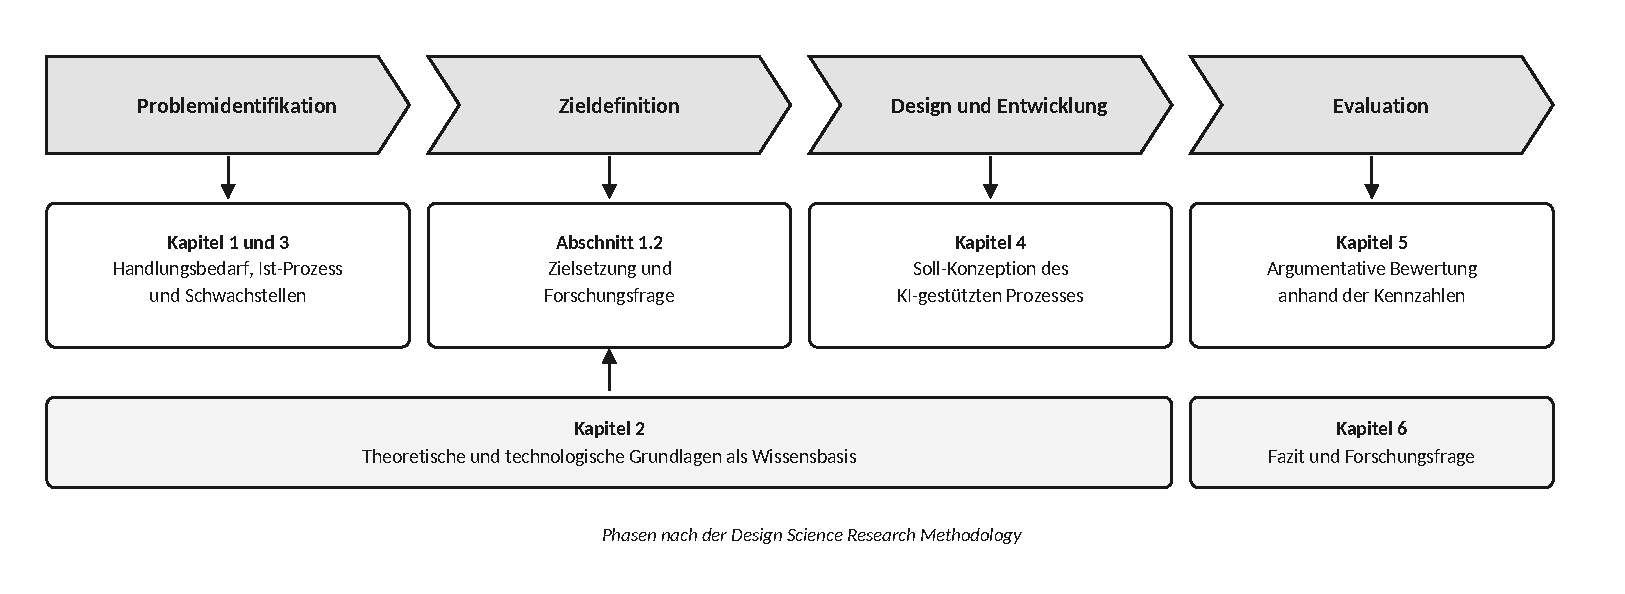
\includegraphics[width=\textwidth]{abb/abb1-dsrm.pdf}
	\caption{Aufbau der Arbeit im DSRM-Phasenmodell}
	\label{fig:dsrm}
	\par\vspace{0.4em}{\footnotesize Dargestellt sind die vier Aktivit"aten, die den Aufbau der Arbeit pr"agen; Demonstration und Kommunikation entfallen aus den oben genannten Gr"unden. Quelle: In Anlehnung an Peffers et al.~(2007), S.~52.}
\end{figure}

Die Grundlagen- und Analysekapitel st\"utzen sich auf eine strukturierte Literaturrecherche in den Datenbanken IEEE Xplore, ACM Digital Library, arXiv und SpringerLink, erg\"anzt um Standardwerke, Rahmenwerke wie ITIL~4 und BPMN~2.0, die einschl\"agigen Rechtsquellen sowie aktuelle Praxisstudien. Die Aufbereitung erfolgt konzeptzentriert nach Webster und Watson, sodass die Argumentation den Themen und nicht den einzelnen Publikationen folgt\footcite[Vgl.][hier S.~xvii]{Webster2002}. Der Suchprozess wird in Anlehnung an vom Brocke et al.~dokumentiert, um die Nachvollziehbarkeit der Quellenauswahl zu sichern; die verwendeten Suchbegriffe, Datenbanken und Auswahlkriterien weist Anhang~I aus.\footcite[Vgl.][hier S.~2211]{VomBrocke2009}

BPMN~2.0 dient als einheitliche Modellierungssprache f\"ur Ist- und Soll-Modell; die Begr\"undung dieser Methodenwahl erfolgt in Abschnitt~2.3. Da keine empirische Erhebung stattfindet, bewertet Kapitel~5 das Konzept argumentativ anhand der in Abschnitt~3.3 definierten Kennzahlen sowie anhand von Befunden der Literatur. Dieses Vorgehen erlaubt Aussagen \"uber die erwartete Wirkungsrichtung, nicht \"uber tats\"achlich erreichte Werte in einer konkreten Organisation, was die Aussagekraft der Evaluation begrenzt. Die f\"ur die Konzeption ben\"otigten Grundlagen entwickelt das folgende Kapitel.

%-----------------------------------
% Kapitel 2: Theoretische und technologische Grundlagen
%-----------------------------------
\section{Theoretische und technologische Grundlagen}

\subsection{IT-Service-Management und Incident Management}

\subsubsection{Einordnung des First-Level-Supports im ITIL-Framework}

% Hier Inhalt einfügen

\subsubsection{Der Incident-Management-Prozess: Ablauf und Beteiligte}

% Hier Inhalt einfügen

\subsection{Künstliche Intelligenz im Unternehmenskontext}

\subsubsection{Abgrenzung von regelbasierten Chatbots zu Large Language Models (LLMs)}

% Hier Inhalt einfügen

\subsubsection{Funktionsweise und Fähigkeiten von LLMs zur Textverarbeitung}

% Hier Inhalt einfügen

\subsubsection{Stand der Forschung: KI im IT-Support und AIOps}

% Hier Inhalt einfügen

\subsection{Prozessmodellierung mit BPMN 2.0}

\subsubsection{Grundlagen der Business Process Model and Notation}

% Hier Inhalt einfügen

\subsubsection{Relevanz für die prozessorientierte Digitalisierung}

% Hier Inhalt einfügen

%-----------------------------------
% Kapitel 3: Ist-Analyse des First-Level-Supports im Incident Management
%-----------------------------------
\section{Ist-Analyse des First-Level-Supports im Incident Management}
\label{istAnalyse}

Kapitel~3 dient der Problemidentifikation im Sinne des in Abschnitt~1.3 dargelegten Vorgehens. Da die Arbeit literaturbasiert angelegt ist, betrachtet sie nicht den Prozess eines einzelnen Unternehmens, sondern einen generischen Referenzprozess, der aus den ITIL-Vorgaben zum Incident Management und zum Service Desk zusammengef\"uhrt wird. Diese Zusammenf\"uhrung stellt eine Eigenleistung dar; die einzelnen Prozessbestandteile sind belegt, ihre Verbindung zu einem durchg\"angigen Ablauf ist es nicht. Abschnitt~3.1 beschreibt den Ablauf in drei Phasen, Abschnitt~3.2 \"uberf\"uhrt ihn in ein BPMN-Modell. Abschnitt~3.3 benennt die Kennzahlen, an denen sich der Prozess messen l\"asst, und Abschnitt~3.4 untersucht Schwachstellen sowie daraus folgende Automatisierungspotenziale.

\subsection{Der First-Level-Support-Prozess nach dem ITIL-Referenzmodell}

Der Ablauf l\"asst sich in drei Phasen gliedern. Abschnitt~3.1.1 behandelt den Ticket-Eingang und die manuelle Triage, Abschnitt~3.1.2 die Informationsbeschaffung und L\"osungsfindung und Abschnitt~3.1.3 die Eskalation in den Second-Level-Support.

\subsubsection{Ticket-Eingang und manuelle Triage}

Meldungen erreichen den Service Desk \"uber mehrere Kan\"ale, die sich im Strukturierungsgrad der \"ubermittelten Angaben unterscheiden. Ein Telefonanruf liefert die Schilderung m\"undlich und erlaubt unmittelbare R\"uckfragen, hinterl\"asst jedoch keine verwertbare Datenstruktur. E-Mails und Chat-Nachrichten liegen als Freitext vor, w\"ahrend ein Self-Service-Portal \"uber Formularfelder bereits eine Vorstrukturierung erzwingt.\\footcite[Vgl.][S.~$\\bullet$]{AXELOS2020} Welche Kan\"ale angeboten werden, richtet sich nach der Nutzergruppe und den vereinbarten Servicezeiten.\\footcite[Vgl.][S.~$\\bullet$]{AXELOS2020} Die Zugangswege bestehen nebeneinander, sodass derselbe Sachverhalt je nach gew\"ahltem Kanal in unterschiedlicher Detailtiefe und Form eintrifft.

Die Erfassung \"uberf\"uhrt die Meldung in das ITSM-Tool. Der Agent legt ein Ticket an und dokumentiert Melder, betroffenen Service, Zeitpunkt sowie die Symptombeschreibung, wobei die Angaben der Anwender h\"aufig unvollst\"andig sind oder Vermutungen \"uber die Ursache anstelle beobachtbarer Symptome enthalten.\\footcite[Vgl.][S.~$\\bullet$]{BeimsZiegenbein} Fehlen entscheidungsrelevante Angaben, stellt der Agent R\"uckfragen, was den Vorgang unterbricht und bei asynchronen Kan\"alen Wartezeiten erzeugt. Mit der Anlage des Tickets beginnt zugleich die Messung der vereinbarten Reaktions- und L\"osungszeiten, weshalb der Erfassungszeitpunkt festgehalten wird.\\footcite[Vgl.][S.~$\\bullet$]{AXELOS2020incident}

Anschlie{\ss}end erfolgt die Triage. Die Kategorisierung ordnet das Ticket \"uber einen mehrstufigen Kategorienbaum einem Service und einer St\"orungsklasse zu, woraus sich die zust\"andige Bearbeitungsgruppe ableitet. Die Priorisierung ergibt sich aus der Einsch\"atzung von Auswirkung und Dringlichkeit, die der Agent anhand der geschilderten Umst\"ande vornimmt.\\footcite[Vgl.][S.~$\\bullet$]{BeimsZiegenbein} Beide Schritte beruhen auf dem Erfahrungswissen des einzelnen Bearbeiters, da sich weder Kategorie noch Priorit\"at unmittelbar aus dem Wortlaut der Meldung ergeben. Bei hohem Meldungsaufkommen findet die Triage unter Zeitdruck statt, weil die Annahme weiterer eingehender Kontakte parallel sicherzustellen ist.\\footcite[Vgl.][S.~$\\bullet$]{AXELOS2020incident} Am Ende der Phase liegt ein erfasstes, kategorisiertes und priorisiertes Ticket vor, dessen weitere Bearbeitung der folgende Abschnitt behandelt.

\subsubsection{Informationsbeschaffung und L\"osungsfindung}

Die Erstdiagnose beginnt mit der Analyse der dokumentierten Symptome. Der Agent pr\"uft, ob die Meldung einem bekannten Fehler entspricht, ob weitere Tickets mit gleichem Muster vorliegen und ob ein laufender Major Incident die St\"orung erkl\"art, dessen Bearbeitung eigenen Regeln folgt.\\footcite[Vgl.][S.~$\\bullet$]{AXELOS2020incident} Erg\"anzend ist zu kl\"aren, ob geplante Wartungsarbeiten oder kurz zuvor durchgef\"uhrte \"Anderungen den geschilderten Effekt hervorrufen, da solche Zusammenh\"ange die weitere Diagnose er\"ubrigen.\\footcite[Vgl.][S.~$\\bullet$]{BeimsZiegenbein} Diese Einordnung entscheidet dar\"uber, ob eine eigenst\"andige Bearbeitung erfolgt oder das Ticket einem bereits laufenden Vorgang zugeordnet wird.

F\"ur die L\"osungsfindung stehen mehrere Informationsquellen bereit. Die Wissensdatenbank enth\"alt dokumentierte L\"osungswege, die Known-Error-Datenbank bekannte Fehler samt zugeh\"origer Workarounds, und die Ticket-Historie erlaubt den Abgleich mit \"ahnlich gelagerten F\"allen.\footcites[Vgl.][S.~$\bullet$]{AXELOS2020incident}[Vgl.][S.~$\bullet$]{BeimsZiegenbein} Die Suche erfolgt manuell \"uber Stichworte, wobei der Treffererfolg von der Formulierung der Suchanfrage und von der Pflege der Best\"ande abh\"angt. Bleibt sie ergebnislos, weitet der Agent die Recherche auf Herstellerdokumentation und weitere allgemeine Quellen aus oder zieht erfahrene Kollegen hinzu. Dieser Schritt beansprucht einen erheblichen Teil der Bearbeitungszeit, insbesondere wenn die Symptombeschreibung des Anwenders von der Terminologie der Wissensartikel abweicht.\footcite[Vgl.][S.~$\bullet$]{BeimsZiegenbein}

F\"uhrt die Recherche zu einem Ergebnis, unternimmt der First Level einen L\"osungsversuch. Typisch sind die Anleitung des Anwenders durch einzelne Schritte, die Anwendung dokumentierter Standardl\"osungen sowie Routinevorg\"ange wie das Zur\"ucksetzen eines Kennworts.\footcites[Vgl.][S.~$\bullet$]{AXELOS2020incident}[Vgl.][S.~$\bullet$]{AXELOS2020} F\"ur wiederkehrende Anliegen halten Organisationen Ablaufbeschreibungen vor, die den Agenten anleiten und ein einheitliches Vorgehen unabh\"angig vom einzelnen Bearbeiter sichern. Gelingt die Wiederherstellung, dokumentiert der Agent das Vorgehen im Ticket, informiert den Anwender und schlie{\ss}t den Vorgang nach dessen Best\"atigung ab.\footcite[Vgl.][S.~$\bullet$]{AXELOS2020} Die Dokumentation dient zugleich als Grundlage f\"ur vergleichbare k\"unftige F\"alle, sofern die L\"osung als Wissensartikel \"ubernommen wird. Bleibt der L\"osungsversuch erfolglos, tritt der Prozess in die Eskalation ein.

\subsubsection{Eskalation in den Second-Level-Support}

Die Weitergabe folgt zwei voneinander unabh\"angigen Logiken. Die funktionale Eskalation greift, wenn dem First Level die fachliche Kompetenz oder die technische Berechtigung zur L\"osung fehlt; das Ticket geht dann an eine Fachgruppe des Second- oder Third-Level-Supports.\footcites[Vgl.][S.~$\bullet$]{AXELOS2020incident}[Vgl.][S.~$\bullet$]{BeimsZiegenbein} Die hierarchische Eskalation richtet sich nicht an Spezialisten, sondern an Entscheidungstr\"ager, und erfolgt, wenn eine Verletzung der SLA-Zielzeiten droht, die Auswirkung der St\"orung hoch ist oder zus\"atzliche Ressourcen freigegeben werden m\"ussen.\footcites[Vgl.][S.~$\bullet$]{BeimsZiegenbein}[Vgl.][S.~$\bullet$]{AXELOS2020incident} Beide Formen k\"onnen denselben Vorgang betreffen. Die Kriterien sind im Vorfeld festgelegt, damit die Entscheidung \"uber eine Weitergabe nicht im Einzelfall neu getroffen werden muss.\footcite[Vgl.][S.~$\bullet$]{BeimsZiegenbein}

Der \"Ubergabe liegt die Zuweisung im ITSM-Tool zugrunde, mit der Zust\"andigkeit und Bearbeitungsstand wechseln. Zur \"Ubergabe geh\"ort neben der Zuweisung eine Zusammenfassung des bisherigen Verlaufs, also der gepr\"uften Annahmen, der durchgef\"uhrten Schritte und ihrer Ergebnisse; bei schwerwiegenden St\"orungen tritt eine m\"undliche Abstimmung hinzu.\footcite[Vgl.][S.~$\bullet$]{AXELOS2020incident} Wie aufw\"andig die weitere Bearbeitung ausf\"allt, h\"angt von der Qualit\"at der bis dahin erfassten Informationen ab, denn eine l\"uckenhafte Dokumentation f\"uhrt zu R\"uckfragen beim Anwender und dazu, dass der Second Level Teile der Diagnose erneut durchf\"uhrt.

Die Zust\"andigkeit f\"ur den Vorgang verbleibt beim Service Desk. Er bleibt Eigent\"umer des Tickets, verfolgt den Bearbeitungsstand, informiert den Anwender \"uber Zwischenst\"ande und nimmt nach der L\"osung dessen Best\"atigung entgegen.\footcite[Vgl.][S.~$\bullet$]{AXELOS2020} Der so beschriebene Ablauf bildet den Referenzprozess dieser Arbeit. Abschnitt~3.2 \"uberf\"uhrt ihn in ein BPMN-Modell.

\subsection{Modellierung des Ist-Zustandes (BPMN-Modell)}

% Hier Inhalt einfuegen

\subsection{Kennzahlen zur Prozessbewertung}

% Hier Inhalt einfuegen

\subsection{Schwachstellenanalyse und Identifikation von Automatisierungspotenzialen}

\subsubsection{Zeitverluste durch manuelle Kategorisierung}

% Hier Inhalt einfügen

\subsubsection{Ineffizienzen durch unstrukturierte Nutzereingaben}

% Hier Inhalt einfügen

%-----------------------------------
% Kapitel 4: Soll-Konzeption des KI-gestützten Incident-Management-Prozesses
%-----------------------------------
\section{Soll-Konzeption des KI-gestützten Incident-Management-Prozesses}
\label{sollKonzeption}

Kapitel~4 tritt in die Redesign-Phase des in Abschnitt~\ref{bpmnDigitalisierung} beschriebenen Lebenszyklus ein und entwickelt damit jenes Artefakt, das Abschnitt~\ref{methodik} als Ziel des gestaltungsorientierten Vorgehens benennt. Grundlage sind die drei in Abschnitt~\ref{schwachstellen} abgeleiteten Automatisierungspotenziale. Abschnitt~\ref{praemissen} kl\"art zun\"achst die Pr\"amissen, denen der neue Ablauf gen\"ugen muss, bevor Abschnitt~\ref{prozessschritte} die einzelnen KI-gest\"utzten Prozessschritte entwickelt. Abschnitt~\ref{sollModell} \"uberf\"uhrt das Ergebnis in ein BPMN-Modell, Abschnitt~\ref{eskalationSoll} behandelt das Eskalationsmanagement. Die Konzeption ist durchgehend hybrid angelegt. Automatisiert wird dort, wo dies fachlich tragf\"ahig ist; die Entscheidung verbleibt beim Menschen, wo Qualit\"at, Recht oder Akzeptanz es verlangen.

\subsection{Prämissen und Anforderungen an den hybriden Workflow}
\label{praemissen}

Abschnitt~\ref{voraussetzungen} behandelt die technischen und organisatorischen Voraussetzungen und leitet aus der Datenschutz-Grundverordnung sowie der KI-Verordnung die rechtlichen Design-Pr\"amissen ab. Abschnitt~\ref{hitl} stellt mit dem Human-in-the-Loop dasjenige Konzept vor, das die Beteiligung des Menschen innerhalb des automatisierten Ablaufs strukturiert.

\subsubsection{Technische und organisatorische Voraussetzungen (inkl. DSGVO und EU AI Act als Design-Prämissen)}
\label{voraussetzungen}

Die KI-Komponenten erg\"anzen das bestehende System, statt an seine Stelle zu treten. Das ITSM-Tool bleibt f\"uhrendes System f\"ur Tickets, Status und Historie, w\"ahrend die Modelle \"uber Schnittstellen darauf zugreifen und ihre Ergebnisse als Vorschlagsfelder in den Vorgang zur\"uckschreiben. Inhaltliche Grundlage maschineller L\"osungsvorschl\"age sind die Wissens- und die Known-Error-Datenbank, deren Pflegezustand die Qualit\"at der Ausgaben unmittelbar begrenzt; wie der Zugriff technisch erfolgt, behandelt Abschnitt~\ref{loesungsvorschlaege}. Eine dritte Voraussetzung betrifft das Betriebsmodell. Ob das Modell im eigenen Rechenzentrum oder in einer Cloud-Umgebung innerhalb der Europ\"aischen Union l\"auft, bestimmt, welche Daten das Unternehmen verlassen, und ist damit bereits eine datenschutzrechtliche Weichenstellung.

Organisatorisch setzt der Betrieb eine gekl\"arte Prozessverantwortung voraus. Die ISO/IEC~20000-1 verlangt ein dokumentiertes Service-Management-System mit festgelegten Rollen, Zielen und Steuerungsmechanismen, in das sich ein KI-gest\"utzter Ablauf einf\"ugen muss.\footcite[Vgl.][S.~$\bullet$]{ISO20000} Iden und Eikebrokk arbeiten in einer systematischen Literaturauswertung Erfolgsfaktoren von ITSM-Einf\"uhrungen heraus, unter denen die Unterst\"utzung durch das Management, die Schulung der Beteiligten und ein schrittweises Vorgehen wiederkehrend genannt w\"urden.\footcite[Vgl.][hier S.~$\bullet$]{IdenEikebrokk2013} Sie lassen sich auf das vorliegende Vorhaben \"ubertragen, da auch hier nicht allein Software eingef\"uhrt, sondern eine eingespielte Arbeitsweise ver\"andert wird. F\"ur die Konzeption folgt daraus, den Prozess stufenweise aktivierbar zu gestalten und den Automatisierungsgrad erst mit belegter Vorschlagsqualit\"at zu erh\"ohen.

Tickets enthalten personenbezogene Daten. Neben der Identit\"at des Melders und seinen Kontaktdaten treten im Freitext regelm\"a{\ss}ig weitere Angaben hinzu, gelegentlich auch solche, die auf gesundheitliche oder arbeitsrechtliche Sachverhalte schlie{\ss}en lassen. Die Verarbeitung unterliegt damit der Datenschutz-Grundverordnung. Aus deren Grunds\"atzen folgt zun\"achst, dass nur die f\"ur die St\"orungsbearbeitung erforderlichen Daten an ein Modell \"ubergeben werden d\"urfen und eine Weiterverwendung zu anderen Zwecken, etwa zur Leistungskontrolle einzelner Agenten, ausscheidet.\footcite[Vgl.][Art.~5 Abs.~1]{DSGVO} Der Datenschutz durch Technikgestaltung verlangt, solche Vorkehrungen bereits in der Architektur vorzusehen.\footcite[Vgl.][Art.~25 Abs.~1]{DSGVO} Hinzu treten die Anforderungen an die Sicherheit der Verarbeitung\footcite[Vgl.][Art.~32]{DSGVO} sowie die Pr\"ufung, ob der Einsatz eine Datenschutz-Folgenabsch\"atzung erfordert.\footcite[Vgl.][Art.~35 Abs.~1]{DSGVO} F\"ur die Prozessgestaltung am folgenreichsten ist Art.~22 Abs.~1 DSGVO, der das Recht gew\"ahrt, nicht einer ausschlie{\ss}lich auf automatisierter Verarbeitung beruhenden Entscheidung unterworfen zu werden, die rechtliche Wirkung entfaltet oder in \"ahnlicher Weise erheblich beeintr\"achtigt.\footcite[Vgl.][Art.~22 Abs.~1]{DSGVO} Bei der \"uberwiegenden Zahl der Support-Vorg\"ange d\"urfte die Vorschrift nicht einschl\"agig sein, da die Zuordnung einer Ticketkategorie niemanden erheblich beeintr\"achtigt. Eine erhebliche Wirkung l\"asst sich umgekehrt dort nicht ausschlie{\ss}en, wo ein Vorgang ohne menschliche Beteiligung abgewiesen oder geschlossen wird und der Melder infolgedessen arbeitsunf\"ahig bleibt. Der Soll-Prozess sieht deshalb vor, abschlie{\ss}ende Entscheidungen \"uber Tickets mit erheblicher Tragweite nicht vollautomatisiert zu treffen. Der Europ\"aische Datenschutzausschuss hebt erg\"anzend hervor, die Verantwortlichkeit verbleibe beim einsetzenden Unternehmen und die Rechtsgrundlage sei f\"ur jede Verarbeitungsphase gesondert zu pr\"ufen.\footcite[Vgl.][S.~$\bullet$]{EDSA2024}

Die KI-Verordnung folgt einem risikobasierten Ansatz und kn\"upft die Pflichten an die Einstufung des jeweiligen Systems. Ein interner Assistent, der Support-Agenten Kategorien, Priorit\"aten und L\"osungswege vorschl\"agt, ist nach der hier vertretenen Einsch\"atzung regelm\"a{\ss}ig nicht als Hochrisiko-System einzuordnen, da er weder \"uber den Zugang zu Besch\"aftigung oder wesentlichen Diensten entscheidet noch in einem der im Anhang der Verordnung aufgef\"uhrten Bereiche zum Einsatz kommt. Einschl\"agig bleibt gleichwohl die Transparenzpflicht, nach der Anwender, die unmittelbar mit dem System interagieren, dar\"uber zu informieren sind, dass sie mit einer KI kommunizieren.\footcite[Vgl.][Art.~50 Abs.~1]{KIVO} Die Anforderungen an die menschliche Aufsicht gelten demgegen\"uber verbindlich nur f\"ur Hochrisiko-Systeme.\footcite[Vgl.][Art.~14]{KIVO} Die vorliegende Arbeit \"ubernimmt sie dennoch als Gestaltungsleitlinie des Soll-Prozesses. Diese \"Ubernahme ist eine bewusste Design-Entscheidung und keine Rechtspflicht; die dort genannten Anforderungen an Verst\"andlichkeit, Eingriffsm\"oglichkeit und kritische Pr\"ufung tragen unabh\"angig von der Einstufung zur Qualit\"atssicherung bei.

Beide Rechtsakte weisen damit in dieselbe Gestaltungsrichtung. Maschinelle Vorarbeit ist zul\"assig, die Letztentscheidung an kritischen Punkten bleibt beim Menschen; das daf\"ur etablierte Konzept behandelt der folgende Abschnitt.

\subsubsection{Das Konzept des \glqq Human-in-the-Loop\grqq{}}
\label{hitl}

Das Konzept des Human-in-the-Loop (HITL) beschreibt Ans\"atze, in denen Mensch und lernendes System innerhalb eines Arbeits- oder Entscheidungsprozesses zusammenwirken, statt einander abzul\"osen. Mosqueira-Rey et al.~ordnen die vorliegenden Auspr\"agungen in einer \"Ubersicht und unterscheiden dabei Active Learning, bei dem das System gezielt nach Annotationen verlange, Interactive Machine Learning mit fortlaufender R\"uckkopplung w\"ahrend des Lernvorgangs sowie Machine Teaching, bei dem Fachexperten ihr Wissen strukturiert einbr\"achten.\footcite[Vgl.][hier S.~$\bullet$]{MosqueiraRey2023} Diese Varianten setzen \"uberwiegend am Training der Modelle an. Die vorliegende Arbeit verwendet den Begriff enger und bezieht ihn auf die Entscheidungsteilhabe im laufenden Betrieb.

Auf die Prozessgestaltung \"ubertragen bedeutet HITL, dass das Modell Vorschl\"age erzeugt und der Agent \"uber deren Verwendung entscheidet. Kategorie, Priorit\"at und L\"osungsweg erreichen den Bearbeiter als vorbelegte Felder, die er best\"atigt, korrigiert oder verwirft; erst diese Handlung erzeugt den verbindlichen Ticketinhalt. Die Rollenverteilung bleibt dadurch eindeutig, denn das Modell wirkt als Assistenzsystem und der Mensch als Entscheidungsinstanz. Zugleich entsteht aus jeder Korrektur eine dokumentierte Abweichung, die sich sp\"ater zur Bewertung der Vorschlagsqualit\"at auswerten l\"asst.

Die Beteiligung des Menschen erf\"ullt ihren Zweck allerdings nur, wenn sie \"uber eine formale Best\"atigung hinausgeht. Die Artikel-29-Datenschutzgruppe h\"alt in ihren Leitlinien fest, eine Aufsicht sei nur dann beachtlich, wenn sie durch eine Person mit entsprechender Befugnis und Kompetenz erfolge, die die Entscheidung tats\"achlich \"uberpr\"ufe und dabei \"uber alle relevanten Informationen verf\"uge; eine routinem\"a{\ss}ige \"Ubernahme des maschinellen Ergebnisses gen\"uge nicht.\footcite[Vgl.][S.~$\bullet$]{WP29Leitlinien2018} Daraus folgt eine praktische Anforderung an die Gestaltung. Werden Agenten an einer Kennzahl gemessen, die kurze Bearbeitungszeiten belohnt, entsteht ein Anreiz, Vorschl\"age ungepr\"uft zu \"ubernehmen; der Prozess liefe dann faktisch vollautomatisiert ab, ohne dass dies im Modell sichtbar w\"urde.

Wie die Entscheidungsknoten auszugestalten sind, l\"asst sich an validierten Leitlinien der Mensch-KI-Interaktion ausrichten. Amershi et al.~empfehlen unter anderem, den Nutzern deutlich zu machen, was das System leisten kann und wo seine Grenzen liegen, die Unsicherheit einer Ausgabe erkennbar zu halten, effiziente Korrekturm\"oglichkeiten vorzusehen und das Systemverhalten nachvollziehbar zu erl\"autern.\footcite[Vgl.][Paper~3, S.~$\bullet$]{Amershi2019} F\"ur den Soll-Prozess bedeutet dies, einen Vorschlag nicht als feststehendes Ergebnis, sondern mit einem Hinweis auf seine Verl\"asslichkeit darzustellen und die Korrektur mit nicht mehr Aufwand zu belegen als die Best\"atigung. Abschnitt~\ref{entscheidungsknoten} greift diese Anforderungen bei der Definition der maschinellen und menschlichen Entscheidungsknoten auf. Auf dieser Pr\"amissenbasis entwickelt der folgende Abschnitt die drei KI-gest\"utzten Prozessschritte.

\subsection{Entwicklung der KI-gestützten Prozessschritte}
\label{prozessschritte}

Die folgenden Abschnitte setzen die drei in Abschnitt~\ref{schwachstellen} abgeleiteten Potenziale in derselben Reihenfolge um. Sie bauen aufeinander auf, denn eine strukturierte Erfassung schafft erst die Grundlage f\"ur eine verl\"assliche Kategorisierung, und beide zusammen bilden die Voraussetzung f\"ur brauchbare L\"osungsvorschl\"age. Abschnitt~\ref{ticketerfassung} behandelt die Erfassung, Abschnitt~\ref{kategorisierungSoll} die Kategorisierung und Priorisierung, Abschnitt~\ref{loesungsvorschlaege} die Generierung von L\"osungsvorschl\"agen.

\begin{figure}[htbp]
	\centering
	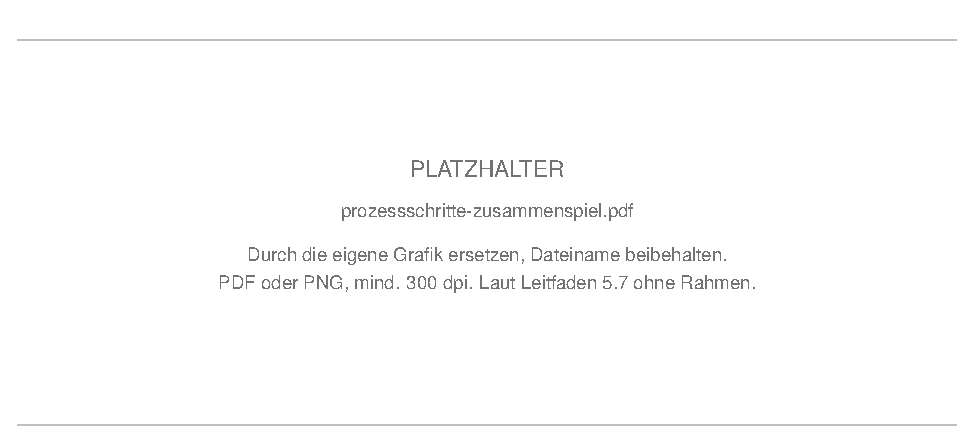
\includegraphics[width=0.95\textwidth]{abbildungen/prozessschritte-zusammenspiel.pdf}
	\caption[Zusammenspiel der drei KI-gest\"utzten Prozessschritte]{Zusammenspiel der drei KI-gest\"utzten Prozessschritte}
	\label{fig:prozessschritte}
\end{figure}

\subsubsection{Automatisierte Ticketerfassung und Intent-Erkennung durch LLMs}
\label{ticketerfassung}

Am Prozessbeginn tritt an die Stelle des starren Formulars ein dialogorientierter Zugang. Der Anwender schildert die St\"orung \"uber Portal oder Chat in eigenen Worten, w\"ahrend ein LLM aus dem Freitext die strukturierten Kernangaben gewinnt, also den betroffenen Service, das beobachtete Symptom, den Wortlaut einer Fehlermeldung, den Zeitpunkt des Auftretens sowie Hinweise auf Dringlichkeit und Reichweite. Parallel dazu bestimmt das Modell das Anliegen. Besonderes Gewicht hat dabei die Unterscheidung zwischen Incident und Service Request, weil sie nach der in Abschnitt~\ref{itilEinordnung} dargelegten Begrifflichkeit \"uber den weiteren Prozesspfad entscheidet. Telefonische Meldungen bleiben davon unber\"uhrt; sie erreichen weiterhin den Agenten, der den Dialog stellvertretend f\"uhrt.

Die Erkennung des Anliegens l\"asst sich als Klassifikationsaufgabe formulieren. Parikh et al.~untersuchen Zero- und Few-Shot-Verfahren zur Intent-Klassifikation und zeigen, dass brauchbare Ergebnisse ohne umfangreiche annotierte Trainingsdaten erreichbar seien.\footcite[Vgl.][hier S.~$\bullet$]{Parikh2023} F\"ur den Support ist das von Belang, weil ein neu aufgesetzter Intent-Katalog andernfalls \"uber Monate hinweg zun\"achst Trainingsmaterial sammeln m\"usste. Die Steuerung erfolgt \"uber strukturierte Prompts, die dem Modell Rolle, Aufgabe und ein festes Ausgabeschema vorgeben, sodass sich das Ergebnis maschinell weiterverarbeiten l\"asst.\footcite[Vgl.][S.~$\bullet$]{Sahoo2024} Der Intent-Katalog leitet sich aus den bestehenden Serviceklassen ab, damit keine zweite, konkurrierende Systematik neben dem gewachsenen Kategorienbaum entsteht. Fehlt eine Pflichtangabe, stellt das System noch im Dialog eine gezielte R\"uckfrage. Die in Abschnitt~\ref{unstrukturiert} beschriebene R\"uckfrageschleife verschwindet damit nicht, sie verlagert sich an den Prozessanfang, wo sie synchron abl\"auft und keine Agentenzeit bindet.

Der Zugang bleibt an die Pr\"amissen aus Abschnitt~\ref{voraussetzungen} gebunden. Der Anwender erf\"ahrt vor dem ersten Austausch, dass er mit einem KI-System kommuniziert, und beh\"alt jederzeit die M\"oglichkeit, in den menschlichen Kanal zu wechseln. Diese Ausweichm\"oglichkeit ist keine Komfortfunktion, sondern Bedingung daf\"ur, dass ein missverstandenes Anliegen nicht im Dialog steckenbleibt. Ebenso gilt die dort begr\"undete Datenminimierung, weshalb dem Modell nur die zur St\"orungsbearbeitung erforderlichen Felder \"ubergeben werden. Das Modell erzeugt zudem keinen verbindlichen Ticketinhalt, sondern einen Entwurf, dessen Felder im weiteren Verlauf best\"atigt werden.

Der erwartete Beitrag liegt in der Vollst\"andigkeit der Tickets bereits zum Zeitpunkt ihrer Erstellung. Angaben, die im Ist-Prozess erst durch asynchrone R\"uckfragen nachgetragen werden, liegen mit der Meldung vor, womit die in Abschnitt~\ref{unstrukturiert} beschriebenen Wartezeiten weitgehend entfallen. Zugleich entsteht ein maschinell verwertbarer Datensatz, auf dem die folgenden Schritte aufsetzen. Wie daraus Kategorie und Priorit\"at abgeleitet werden, behandelt der folgende Abschnitt.

\subsubsection{KI-gestützte Kategorisierung und Priorisierung}
\label{kategorisierungSoll}

Auf Grundlage des strukturierten Tickets schl\"agt das System Kategorie und Priorit\"at vor. Die Kategorie ergibt sich aus dem geschilderten Sachverhalt und dem betroffenen Service, die Priorit\"at aus den bei der Erfassung gewonnenen Indikatoren f\"ur Auswirkung und Dringlichkeit, die nach der in Abschnitt~\ref{incidentProzess} dargestellten Matrix zusammengef\"uhrt werden. Beide Vorschl\"age erreichen den Agenten gemeinsam mit dem Ticket und nicht als nachgelagerter Arbeitsschritt; sie ersetzen die Eingabefelder nicht, sondern belegen sie vor.

Die Modellwahl f\"allt f\"ur die beiden Aufgaben unterschiedlich aus. F\"ur die vielklassige Kategorisierung sprechen die in Abschnitt~\ref{aiopsStand} referierten Befunde f\"ur feinabgestimmte Encoder-Modelle, die generative Modelle in dieser Aufgabe \"ubertreffen k\"onnten und zugleich mit geringerem Rechenaufwand auskommen.\footcites[Vgl.][S.~$\bullet$]{Autoren2024}[][S.~$\bullet$]{Jurkus2026} Eine aktuelle Vergleichsuntersuchung stellt klassische Verfahren des maschinellen Lernens und sprachmodellbasierte Ans\"atze f\"ur Klassifikation und Zuweisung von Tickets gegen\"uber und best\"atigt die Eignung beider Familien f\"ur diesen Aufgabentyp.\footcite[Vgl.][S.~$\bullet$]{Autoren2025} Die Konzeption sieht deshalb eine Arbeitsteilung vor. Ein feinabgestimmtes Encoder-Modell bestimmt die Kategorie, w\"ahrend das LLM die Priorit\"atsindikatoren aus dem Freitext ableitet und eine kurze, f\"ur den Agenten nachvollziehbare Begr\"undung des Vorschlags formuliert. F\"ur den Betrieb hat diese Trennung den Vorzug, dass sich beide Komponenten unabh\"angig voneinander austauschen und bewerten lassen. Da die Priorit\"at aus mehreren Teilurteilen entsteht, l\"asst sich dieser Schritt in eine Folge von Zwischenschritten zerlegen; Wei et al.~zeigen, dass eine derart schrittweise Aufgabenstellung die Bearbeitung mehrstufiger Entscheidungen durch Sprachmodelle verbessere.\footcite[Vgl.][S.~$\bullet$]{Wei2022}

Beide Vorschl\"age erscheinen im Bearbeitungsfenster als vorbelegte Felder mit einer Angabe zur Konfidenz. Der Agent \"ubernimmt sie mit einem Klick oder \"uberschreibt sie; eine \"Ubernahme ohne Anzeige der Konfidenz scheidet nach den Pr\"amissen aus Abschnitt~\ref{hitl} aus. Jede Korrektur wird protokolliert und steht als R\"uckmeldung f\"ur die sp\"atere Nachjustierung des Kategorisierungsmodells zur Verf\"ugung. Damit entsteht ein geschlossener Kreis, in dem gerade jene F\"alle dokumentiert werden, in denen das Modell danebenliegt.

Der erwartete Beitrag betrifft unmittelbar die in Abschnitt~\ref{manuelleKategorisierung} beschriebene Schwachstelle. Trifft die vorgeschlagene Kategorie zu, entf\"allt die manuelle Suche im Kategorienbaum, und die Zuweisung an eine unzust\"andige Gruppe wird seltener, womit Ping-Pong-Eskalationen und die daraus folgende Verl\"angerung der Mean Time to Resolve zur\"uckgehen. Trifft sie nicht zu, kostet die Korrektur nicht mehr Zeit als die bisherige manuelle Eingabe. Hinzu tritt eine gleichm\"a{\ss}igere Zuordnung, da der Vorschlag nicht vom Erfahrungsstand des einzelnen Bearbeiters abh\"angt. Wie aus dem kategorisierten Ticket ein L\"osungsweg entsteht, behandelt der folgende Abschnitt.

\subsubsection{Generierung von Lösungsvorschlägen und Self-Service-Antworten}
\label{loesungsvorschlaege}

Der dritte Schritt richtet sich an zwei Empf\"anger. Gegen\"uber dem Agenten wirkt das System assistiv, indem es zum Ticket passende L\"osungswege vorschl\"agt und die zugeh\"origen Fundstellen benennt. Gegen\"uber dem Anwender tritt es bei klar umgrenzten Standardanliegen selbst in Erscheinung und beantwortet die Meldung unmittelbar, sodass ein Teil der Vorg\"ange den Agenten nicht erreicht. Beide Richtungen nutzen denselben technischen Mechanismus und unterscheiden sich im Grad der menschlichen Beteiligung.

Den Kern bildet die Retrieval-Augmented Generation (RAG). Das Modell beantwortet die Anfrage nicht aus dem im Training erworbenen Wissen, sondern auf Grundlage von Inhalten, die zuvor gezielt aus einem externen Bestand abgerufen werden. Lewis et al.~verbinden dazu ein Retrieval-Modul mit einem generativen Modell und zeigen, dass sich wissensintensive Aufgaben auf diese Weise bearbeiten lassen, ohne das ben\"otigte Wissen in den Modellparametern vorhalten zu m\"ussen.\footcite[Vgl.][S.~$\bullet$]{Lewis2020} Gao et al.~ordnen die inzwischen vorliegenden Architekturvarianten und beschreiben, wie sich Abruf, Aufbereitung und Erzeugung unterschiedlich verzahnen lie{\ss}en.\footcite[Vgl.][S.~$\bullet$]{Gao2023} Im vorliegenden Entwurf bilden die Wissens- und die Known-Error-Datenbank den abgerufenen Bestand. Da der Abruf \"uber Bedeutungs\"ahnlichkeit erfolgt, greift er auch dann, wenn der Anwender andere Begriffe verwendet als die Autoren der Wissensartikel; das in Abschnitt~\ref{unstrukturiert} beschriebene Stichwortproblem entf\"allt. Die Bindung an abgerufene Quellen begrenzt zugleich die Neigung des Modells, plausible, aber unzutreffende Aussagen zu erzeugen, und erlaubt es, jeder Antwort die verwendete Fundstelle beizugeben; die verbleibenden Grenzen behandelt Abschnitt~\ref{herausforderungen}.

F\"ur den Support liegen erste Anwendungen vor. Toro Isaza et al.~beschreiben ein RAG-gest\"utztes Empfehlungssystem f\"ur die Incident-Bearbeitung im IT-Support.\footcite[Vgl.][S.~$\bullet$]{ToroIsaza2024} Baqar \"ubertr\"agt den Ansatz auf Ticket- und Repository-Daten und zeigt, dass auch kleinere, lokal betreibbare Modelle f\"ur die Aufgabe in Betracht k\"amen.\footcite[Vgl.][S.~$\bullet$]{Baqar2025} Letzteres ber\"uhrt unmittelbar die in Abschnitt~\ref{voraussetzungen} getroffene Weichenstellung zum Betriebsmodell, da ein lokal betriebenes Modell den Abfluss personenbezogener Ticketinhalte an Dritte vermeidet.

Die Beteiligung des Menschen f\"allt je nach Empf\"anger unterschiedlich aus. Ein L\"osungsvorschlag an den Agenten bleibt stets Vorschlag; er wird angezeigt und nicht ausgef\"uhrt, und die Entscheidung \"uber seine Verwendung liegt beim Bearbeiter. Eine Antwort unmittelbar an den Anwender ohne vorherige menschliche Pr\"ufung sieht der Entwurf nur f\"ur einen zuvor festgelegten Katalog risikoarmer Standardf\"alle vor, etwa f\"ur Anleitungen ohne Eingriff in produktive Systeme. Jede solche Antwort tr\"agt den Hinweis auf ihre maschinelle Erzeugung und die M\"oglichkeit, den Vorgang unmittelbar an einen Agenten zu \"ubergeben. Nach welchen Kriterien die Grenze dieses Katalogs verl\"auft, behandelt Abschnitt~\ref{fallback}.

Der erwartete Beitrag verteilt sich auf beide Richtungen. Die assistive Nutzung verk\"urzt die in Abschnitt~\ref{loesungsfindung} beschriebene Recherche und erh\"oht die Wahrscheinlichkeit, dass ein Fall im Erstkontakt gel\"ost wird, was auf die First Contact Resolution Rate wirkt. Der Self-Service-Anteil senkt das Ticketaufkommen bei Standardanliegen und schafft Bearbeitungszeit f\"ur F\"alle, die tats\"achlich Fachwissen erfordern. Wie sich die drei Schritte in den Gesamtablauf einf\"ugen, zeigt das Soll-Modell im folgenden Abschnitt.

\subsection{Modellierung des Soll-Zustandes (BPMN-Modell)}
\label{sollModell}

\subsubsection{Darstellung der neuen Prozessarchitektur}
\label{prozessarchitektur}

% Hier Inhalt einfügen: BPMN-Diagramm des Soll-Prozesses

\subsubsection{Definition der maschinellen und menschlichen Entscheidungsknoten}
\label{entscheidungsknoten}

% Hier Inhalt einfügen

\subsection{Eskalationsmanagement im Soll-Prozess}
\label{eskalationSoll}

\subsubsection{Kriterien für den automatisierten Fallback zum menschlichen Bearbeiter}
\label{fallback}

% Hier Inhalt einfügen

\subsubsection{Übergabe und Kontexttransfer an den Second-Level-Support}
\label{kontexttransfer}

% Hier Inhalt einfügen

%-----------------------------------
% Kapitel 5: Evaluation und zukünftige Technologiepotenziale
%-----------------------------------
\section{Evaluation und zukünftige Technologiepotenziale}
\label{evaluation}

Kapitel~5 tritt in die Evaluationsphase des in Abschnitt~\ref{methodik} dargelegten Vorgehens ein. Abschnitt~\ref{wuerdigung} w\"urdigt das in Kapitel~\ref{sollKonzeption} entwickelte Artefakt kritisch, indem er die erwarteten Wirkungen an den Kennzahlen aus Abschnitt~\ref{kennzahlen} pr\"uft und ihnen die Risiken gegen\"uberstellt. Abschnitt~\ref{ausblick} richtet den Blick auf Entwicklungen, die \"uber den vorliegenden Entwurf hinausweisen. Da keine empirische Erhebung stattfindet, handelt es sich durchgehend um erwartete und nicht um gemessene Wirkungen; die Aussagen betreffen Richtungen, nicht Betr\"age.

\subsection{Kritische Würdigung des Soll-Konzeptes}
\label{wuerdigung}

Die Evaluation im Sinne der Design Science Research Methodology vergleicht das entwickelte Artefakt mit den Zielen, die zu Beginn festgelegt wurden\footcite[Vgl.][S.~56]{Peffers2007}. Venable, Pries-Heje und Baskerville ordnen Evaluationen in der gestaltungsorientierten Forschung nach zwei Dimensionen, n\"amlich dem Zweck, der formativ oder summativ sein kann, und dem Paradigma, das artifiziell oder naturalistisch angelegt ist\footcite[Vgl.][hier S.~77]{Venable2016}. Die nachfolgende W\"urdigung ist in dieser Systematik eine formative Evaluation im artifiziellen Paradigma und findet ex ante statt, also vor einer Umsetzung. Sie pr\"uft das Artefakt argumentativ gegen die Anforderungen und die Befunde der Literatur, nicht im Einsatz bei Anwendern. Das ist keine Notl\"osung, sondern der f\"ur ein noch nicht implementiertes Artefakt vorgesehene Typ; seine Grenze liegt darin, dass er \"uber die Wirkungsrichtung Auskunft gibt und nicht \"uber die Wirkungsh\"ohe. Die Forschungsfrage aus Abschnitt~\ref{zielsetzung} nennt vier Anforderungen, n\"amlich Effizienz, Qualit\"at, Datenschutz und Kontrolle. \autoref{tab:erfuellung} stellt ihnen die Elemente des Soll-Konzeptes gegen\"uber und weist aus, in welchem Ma{\ss}e die Anforderung als erf\"ullt gelten kann.

\begin{table}[htbp]
	\centering
	\caption{Anforderungen der Forschungsfrage und ihre Umsetzung im Soll-Konzept}
	\label{tab:erfuellung}
	\begin{tabularx}{\textwidth}{@{}p{2.1cm}>{\raggedright\arraybackslash}X>{\raggedright\arraybackslash}X@{}}
		\toprule
		Anforderung & Umsetzung im Konzept & Erf\"ullungsgrad \\
		\midrule
		Effizienz & Dialogorientierte Erfassung, maschinelle Kategorisierung und Priorisierung, abrufgest\"utzte L\"osungsvorschl\"age (Abschnitt~\ref{prozessschritte}) & Wirkungsrichtung f\"ur alle vier Kennzahlen hergeleitet, H\"ohe der Wirkung nicht gemessen \\
		Qualit\"at & Konfidenzschwelle vor der \"Ubernahme, Begr\"undungspflicht des Vorschlags, Protokollierung jeder Korrektur (Abschnitte~\ref{kategorisierungSoll} und \ref{fallback}) & konzeptionell verankert, Wirksamkeit von der Kalibrierung des Modells abh\"angig \\
		Datenschutz & Positivliste f\"ur vollautomatisierte Antworten, Ausschluss automatisierter Bearbeitung bei sensiblen Inhalten, Zweckbindung der Korrekturprotokolle (Abschnitte~\ref{voraussetzungen} und \ref{fallback}) & konzeptionell verankert, Umsetzung setzt organisatorische Festlegungen voraus \\
		Kontrolle & Gestaffelte Beteiligung des Menschen, menschliche Entscheidungsknoten, Eskalationsentscheidung beim Agenten (Abschnitte~\ref{hitl} und \ref{entscheidungsknoten}) & im Prozessmodell abgebildet, Wirksamkeit von der tats\"achlichen Pr\"ufung durch die Agenten abh\"angig \\
		\bottomrule
	\end{tabularx}
\end{table}

Die Matrix zeigt ein einheitliches Muster. Alle vier Anforderungen sind im Prozessmodell verankert und nicht als begleitende Ma{\ss}nahmen angef\"ugt; keine von ihnen ist jedoch allein durch die Konzeption eingel\"ost, da ihre Wirksamkeit von Gr\"o{\ss}en abh\"angt, die erst im Betrieb entstehen. Abschnitt~\ref{effizienz} leitet die erwarteten Effizienzwirkungen f\"ur die vier Kennzahlen ab und benennt dabei auch gegenl\"aufige Effekte. Abschnitt~\ref{herausforderungen} behandelt anschlie{\ss}end die Herausforderungen, die dem Konzept Grenzen setzen.

\subsubsection{Erwartete Effizienzsteigerungen anhand der in Abschnitt~3.3 definierten Kennzahlen}
\label{effizienz}

F\"ur die First Contact Resolution Rate wirken zwei Mechanismen in dieselbe Richtung. Die bedeutungsbasierte Suche aus Abschnitt~\ref{loesungsvorschlaege} findet Wissensartikel auch dann, wenn der Anwender eine andere Terminologie verwendet als deren Autoren, womit das in Abschnitt~\ref{unstrukturiert} beschriebene Stichwortproblem entf\"allt und mehr F\"alle bereits im Erstkontakt l\"osbar werden. Hinzu tritt der Self-Service-Pfad, der Standardanliegen ohne Beteiligung eines Agenten abschlie{\ss}t und sie damit definitionsgem\"a{\ss} im ersten Kontakt l\"ost.

Die Kennzahl reagiert auf diese Ver\"anderung allerdings nicht eindeutig. Werden Standardf\"alle automatisiert abgeschlossen, verbleiben im Agenten-Kanal \"uberproportional die schwierigeren Vorg\"ange, deren L\"osung im Erstkontakt seltener gelingt. Die f\"ur diesen Kanal gemessene FCR kann dadurch sinken, obwohl die Leistung des Gesamtprozesses steigt. Eine belastbare Interpretation setzt deshalb voraus, dass die Kanalverschiebung mit ausgewiesen wird, etwa durch getrennte Betrachtung von Self-Service- und Agenten-Pfad neben einem zusammengefassten Wert \"uber beide.

Bei der Mean Time to Resolve greifen vier Mechanismen ineinander. Die manuelle Triage aus Abschnitt~\ref{manuelleKategorisierung} entf\"allt als eigener Zeitblock, sofern der Vorschlag angenommen wird. Die asynchronen R\"uckfrageschleifen verk\"urzen sich, weil die Erfassung fehlende Angaben bereits im Dialog erhebt. Eine treffendere Kategorisierung senkt die Zahl der Fehlzuweisungen und damit der Ping-Pong-Eskalationen. Der Kontexttransfer aus Abschnitt~\ref{kontexttransfer} beschleunigt schlie{\ss}lich die \"Ubergabe an den Second Level, weil dort weniger nachgefragt und weniger doppelt diagnostiziert wird.

Einen empirischen Anhaltspunkt f\"ur die Gr\"o{\ss}enordnung liefert die bereits in Abschnitt~\ref{ausgangssituation} herangezogene Untersuchung, die f\"ur LLM-gest\"utzte Assistenz eine Zunahme der je Stunde gel\"osten F\"alle um 15~Prozent ausweist und den st\"arksten Effekt bei unerfahrenen Mitarbeitenden feststellt\footcite[Vgl.][S.~890]{Brynjolfsson2025}. \"Ubertragen auf den vorliegenden Entwurf legt dieser Befund nahe, dass der Nutzen dort am gr\"o{\ss}ten ausf\"allt, wo die Fluktuation hoch und der Anteil neu eingearbeiteter Agenten entsprechend gro{\ss} ist. Zugleich mahnt die Herkunft des Befundes zur Zur\"uckhaltung, denn er stammt aus einem Kundenservice-Umfeld und nicht aus einem an ITIL ausgerichteten Service Desk.

Die First Level Resolution Rate d\"urfte am deutlichsten zunehmen, da beide Schwachstellenfelder unmittelbar auf sie wirken. Treffendere Kategorien verringern die Zahl der Vorg\"ange, die allein wegen einer Fehlzuordnung den First Level verlassen, und abrufgest\"utzte L\"osungsvorschl\"age erweitern den Kreis der dort abschlie{\ss}bar bearbeitbaren F\"alle. Gegenl\"aufig wirkt allein die in Abschnitt~\ref{fallback} vorgesehene Eskalation bei unzureichender Konfidenz, die Vorg\"ange bewusst fr\"uher weitergibt. Da f\"ur die FLR kein \"offentlich belegter Vergleichswert vorliegt, ist ihre Entwicklung ausschlie{\ss}lich gegen den Ausgangswert der jeweiligen Organisation zu beurteilen.

Beide Wirkungen h\"angen vom Kanalmix ab. Da telefonische Meldungen nach Abschnitt~\ref{prozessarchitektur} weiterhin vom Agenten erfasst werden, f\"allt der Erfassungsgewinn bei hohem Telefonanteil geringer aus. Das Ticketvolumen pro Agent d\"urfte steigen, da Erfassung und Triage weitgehend entfallen und die Recherche k\"urzer ausf\"allt. Die in Abschnitt~\ref{kennzahlen} formulierte Einschr\"ankung gilt hier jedoch versch\"arft. Die Kennzahl ist ohne Betrachtung des Ticketmix wenig aussagekr\"aftig, und genau diesen Mix ver\"andert der Self-Service-Pfad, indem er einfache Vorg\"ange herausl\"ost. Ein gestiegener Wert w\"are daher nicht ohne Weiteres als Produktivit\"atsgewinn zu lesen; ebenso denkbar ist, dass die verbleibenden F\"alle je Vorgang mehr Zeit beanspruchen und die Kennzahl trotz besserer Werkzeuge stagniert.

S\"amtliche Aussagen dieses Abschnitts beschreiben Wirkungsrichtungen, die sich aus der Konstruktion des Prozesses ergeben, und keine gemessenen Effekte. Die in Abschnitt~\ref{kennzahlen} referierten Vergleichswerte taugen als Bezugsrahmen f\"ur eine sp\"atere Einordnung, nicht als Prognose f\"ur eine konkrete Organisation\footcites[Vgl.][o.~S.\isdot]{Rumburg2011}[][o.~S.\isdot]{Rumburg2018}[][o.~S.]{MetricNet2020}. Eine belastbare Quantifizierung setzt eine Pilotierung mit Vorher-Nachher-Messung voraus, in der die vier Kennzahlen vor und nach Aktivierung der KI-Komponenten unter sonst vergleichbaren Bedingungen erhoben werden. Diese Grenze ist der literaturbasierten Anlage der Arbeit geschuldet.

Effizienz ist zudem ein Verh\"altnis von Ertrag und Aufwand, weshalb die bislang betrachtete Ertragsseite allein kein Urteil erlaubt. Auf der Aufwandsseite stehen vier Bl\"ocke. Einmalig f\"allt die Einf\"uhrung an, also die Anbindung an das ITSM-System, die Feinabstimmung des Kategorisierungsmodells auf den vorhandenen Ticketbestand und die Aufbereitung der Wissensdatenbank f\"ur den Abruf. Laufend entstehen Betriebskosten f\"ur die Modellnutzung, die bei einem extern bezogenen Dienst mit der Zahl der Anfragen wachsen und bei lokalem Betrieb als Vorhaltung von Rechenkapazit\"at anfallen. Hinzu tritt der fortlaufende Pflegeaufwand, da der in Abschnitt~\ref{loesungsvorschlaege} beschriebene Abruf nur so gut ist wie der Wissensbestand, auf den er zugreift. Schlie{\ss}lich verursachen die Schulung der Agenten und die in Abschnitt~\ref{voraussetzungen} genannten organisatorischen Festlegungen Aufwand, der nicht technischer Natur ist.

Eine Bezifferung dieser Bl\"ocke ist ohne konkreten Organisationsbezug nicht m\"oglich, da sie vom Ticketvolumen, vom gew\"ahlten Betriebsmodell und vom Zustand der vorhandenen Wissensdatenbank abh\"angt. Festhalten l\"asst sich jedoch die Struktur des Zusammenhangs: Der Einf\"uhrungsaufwand f\"allt unabh\"angig vom Ticketvolumen an, w\"ahrend die Entlastung mit ihm w\"achst. Der Aufbau lohnt sich daher erst oberhalb eines Volumens, das im Einzelfall zu bestimmen ist. Den erwarteten Nutzeffekten stehen \"uberdies Risiken gegen\"uber, die der folgende Abschnitt behandelt.

\subsubsection{Herausforderungen (Halluzinationen von LLMs, Datenschutz, IT-Sicherheit, Akzeptanz)}
\label{herausforderungen}

Sprachmodelle erzeugen Inhalte, die durch die zugrunde liegenden Quellen nicht gedeckt sind. Zhao et al.~unterscheiden intrinsische Halluzinationen, die der bereitgestellten Eingabe widersprechen, von extrinsischen, die sich an ihr nicht \"uberpr\"ufen lassen\footcite[Vgl.][S.~59]{Zhao2023}. F\"ur den Support wiegt die erste Kategorie schwerer, weil ein L\"osungsvorschlag an den abgerufenen Wissensartikeln zu messen ist, die dem Modell als Eingabe vorliegen.

Im Soll-Prozess wirkt sich das an zwei Stellen aus. Ein unzutreffender, aber plausibel formulierter L\"osungsvorschlag kann einen Agenten zu einem Eingriff veranlassen, der die St\"orung versch\"arft. Eine fehlerhafte Self-Service-Antwort erreicht den Anwender ohne Zwischenpr\"ufung. Das Konzept begegnet dem mit der Bindung an abgerufene Wissensartikel, der Ausweisung der Fundstellen, der Pr\"ufung durch den Agenten und der Beschr\"ankung des Self-Service auf eine Positivliste. Diese Ma{\ss}nahmen greifen ineinander, beseitigen das Problem jedoch nicht. Die Quellenbindung senkt die Wahrscheinlichkeit unzutreffender Aussagen, schlie{\ss}t sie aber nicht aus, etwa wenn abgerufene Artikel veraltet sind oder das Modell sie unzutreffend verdichtet. Die menschliche Pr\"ufung wiederum wirkt nur, soweit sie tats\"achlich stattfindet; der in Abschnitt~\ref{fallback} herangezogene Befund zur schlecht kalibrierten Nutzung algorithmischer Vorschl\"age gilt hier unver\"andert.\footcite[Vgl.][S.~1]{GreenChen2019}

Das zweite Feld betrifft den Datenschutz. Anwender liefern im Freitext regelm\"a{\ss}ig Angaben mit, nach denen niemand gefragt hat und deren Sensibilit\"at sich erst bei der Verarbeitung zeigt. Da die Erfassung nach Abschnitt~\ref{ticketerfassung} gerade auf offene Schilderungen setzt, beg\"unstigt der Entwurf dieses Verhalten sogar. Bei externem Modellbetrieb treten Fragen der \"Ubermittlung, der Zweckbindung und der Speicherdauer hinzu, f\"ur die Abschnitt~\ref{voraussetzungen} den rechtlichen Rahmen benannt hat. Offen bleiben mehrere Punkte, die eine Umsetzung zu kl\"aren h\"atte. Das Dialogdesign w\"are so anzulegen, dass es nicht mehr Angaben hervorruft als erforderlich. F\"ur Dialoghistorien und Modellprotokolle w\"aren L\"oschfristen festzulegen. Vor Inbetriebnahme ist eine Datenschutz-Folgenabsch\"atzung durchzuf\"uhren, sofern die Verarbeitung voraussichtlich ein hohes Risiko f\"ur die Rechte und Freiheiten nat\"urlicher Personen zur Folge hat; die Aufsichtsbeh\"orden f\"uhren hierzu Listen der Verarbeitungsvorg\"ange, f\"ur die eine solche Absch\"atzung verpflichtend ist\footcites[Vgl.][Art.~35 Abs.~1]{DSGVO}[][Art.~35 Abs.~4]{DSGVO}. Die Liste der Datenschutzkonferenz f\"ur den nicht-\"offentlichen Bereich f\"uhrt unter Nr.~11 den Einsatz k\"unstlicher Intelligenz zur Verarbeitung personenbezogener Daten auf, soweit er die Interaktion mit den Betroffenen steuert, und nennt als typisches Einsatzfeld ausdr\"ucklich den Kundensupport mittels k\"unstlicher Intelligenz\footcite[Vgl.][Nr.~11, S.~3]{DSK2018}. Die dialogorientierte Erfassung des Soll-Prozesses entspricht dieser Beschreibung, auch wenn die Betroffenen hier Besch\"aftigte und keine Kunden sind; eine Datenschutz-Folgenabsch\"atzung ist deshalb vor Inbetriebnahme durchzuf\"uhren. F\"ur die Korrekturprotokolle ist zus\"atzlich Nr.~8 der Liste einschl\"agig, die umfangreiche Verarbeitungen von Daten \"uber das Verhalten Besch\"aftigter erfasst, sofern diese zur Bewertung der Arbeitst\"atigkeit so eingesetzt werden k\"onnen, dass die Betroffenen erheblich beeintr\"achtigt werden\footcite[Vgl.][Nr.~8, S.~3]{DSK2018}. Ob dieser Tatbestand greift, h\"angt vom Umfang der Protokollierung und von ihrer Verwendbarkeit ab; die in Abschnitt~\ref{voraussetzungen} festgelegte Zweckbindung setzt genau an dieser Stelle an. Diese Punkte sind im vorliegenden Konzept als Anforderung benannt, nicht ausgearbeitet.

Das dritte Feld betrifft die IT-Sicherheit und folgt unmittelbar aus der Architektur des Soll-Prozesses. Das Sprachmodell verarbeitet Freitext, den ein Anwender verfasst, und ruft zus\"atzlich Inhalte aus der Wissensdatenbank ab. Beide Wege sind Einfallstore f\"ur Prompt Injection, also f\"ur Eingaben, die das Verhalten des Modells in unbeabsichtigter Weise ver\"andern. Die OWASP Foundation f\"uhrt diese Schwachstelle als gr\"o{\ss}tes Risiko von Anwendungen mit Sprachmodellen und unterscheidet die direkte Einschleusung \"uber die Nutzereingabe von der indirekten \"uber abgerufene Inhalte; abrufgest\"utzte Verfahren beseitigten das Problem nicht\footcite[Vgl.][o.~S.]{OWASP2025}. F\"ur den vorliegenden Prozess bedeutet dies zweierlei. Eine St\"orungsmeldung k\"onnte Anweisungen enthalten, die auf eine unzutreffend hohe Priorit\"at oder auf die Ausgabe von Inhalten zielen, die dem Melder nicht zustehen. Und ein manipulierter Wissensartikel w\"urde \"uber den Abruf in die Antwort gelangen, ohne dass die Manipulation im Dialog sichtbar w\"urde. Der Entwurf begegnet dem an drei Stellen, die bereits angelegt sind: Die Positivliste begrenzt die vollautomatisierte Beantwortung auf einen definierten Katalog, die menschliche Pr\"ufung an den \"ubrigen Knoten f\"angt auff\"allige Ausgaben ab, und die Konfidenzanzeige macht unsichere Vorschl\"age erkennbar. Hinzutreten m\"ussen eine als unsicher behandelte Trennung von Nutzereingabe und Systemanweisung sowie ein Freigabeprozess f\"ur Wissensartikel, der festlegt, wer Inhalte einstellen darf. Damit ist das Risiko begrenzt, aber nicht beseitigt.

Das vierte Feld betrifft die Akzeptanz, wobei zwei Nutzergruppen zu unterscheiden sind. F\"ur die Agenten bietet die Unified Theory of Acceptance and Use of Technology (UTAUT) einen Analyserahmen; Venkatesh et al.~f\"uhren Leistungserwartung, Aufwandserwartung, sozialen Einfluss und erleichternde Bedingungen als Bestimmungsgr\"o{\ss}en der Nutzungsabsicht an\footcite[Vgl.][hier S.~447]{Venkatesh2003}. Die Leistungserwartung d\"urfte hier ambivalent ausfallen, da ein System, das Kategorien vorschl\"agt und Korrekturen protokolliert, zugleich als Entlastung und als Kontrolle der eigenen Arbeit wahrgenommen werden kann. Hinzu treten zwei gegenl\"aufige Fehlhaltungen. Dietvorst, Simmons und Massey zeigen, dass Personen algorithmische Verfahren nach beobachteten Fehlern mieden, selbst wenn diese dem menschlichen Urteil \"uberlegen blieben\footcite[Vgl.][hier S.~115]{Dietvorst2015}. Parasuraman und Manzey beschreiben umgekehrt die unkritische \"Ubernahme automatisierter Ausgaben infolge nachlassender Aufmerksamkeit\footcite[Vgl.][hier S.~381]{ParasuramanManzey2010}. Beide Haltungen f\"uhren zu unerw\"unschten Ergebnissen, die sich nicht allein technisch auffangen lassen; erforderlich sind Schulung, ein offener Umgang mit Fehlern des Systems und die in Abschnitt~\ref{entscheidungsknoten} vorgesehene Konfidenzanzeige. F\"ur die Anwender stellt sich die Frage anders. Ein Self-Service l\"asst sich als Beschleunigung erleben oder als Abschottung der IT-Organisation, je nachdem, wie leicht ein Mensch erreichbar bleibt. Die in Abschnitt~\ref{ticketerfassung} vorgesehene Ausweichoption ist damit weniger eine Komfortfunktion als eine Bedingung der Akzeptanz.

Die vier Felder begrenzen den erreichbaren Automatisierungsgrad, ohne die hybride Architektur selbst zu ber\"uhren, da sie s\"amtlich an der Verl\"asslichkeit maschineller Ausgaben ansetzen und nicht an der Aufteilung zwischen Maschine und Mensch. Alle vier begrenzen jedoch, wie weit die Automatisierung tragen kann, und zwar unabh\"angig davon, wie leistungsf\"ahig die eingesetzten Modelle sind. Die hybride Architektur erweist sich damit nicht als \"Ubergangsl\"osung auf dem Weg zur Vollautomatisierung, sondern als Konsequenz aus diesen Grenzen. Welche technologischen Entwicklungen diese Grenzen verschieben k\"onnten, behandelt der folgende Abschnitt.

\subsection{Ausblick auf zukünftige Entwicklungen im IT-Support}
\label{ausblick}

Das in Kapitel~\ref{sollKonzeption} entwickelte Konzept beschreibt den Stand dessen, was sich gegenw\"artig verantwortbar umsetzen l\"asst. Zwei Entwicklungslinien k\"onnten die Aufgabenteilung zwischen Mensch und System k\"unftig weiter verschieben. Abschnitt~\ref{kiAgenten} betrachtet den \"Ubergang von assistierenden zu agentischen Systemen, Abschnitt~\ref{predictive} die Verlagerung von der reaktiven zur vorausschauenden St\"orungsbearbeitung.

\subsubsection{Von assistierenden LLMs zu autonomen KI-Agenten}
\label{kiAgenten}

Das Soll-Konzept nutzt Sprachmodelle assistierend. Sie erzeugen Vorschl\"age, w\"ahrend der Prozessrahmen den Ablauf und der Mensch die Entscheidung bestimmt. KI-Agenten gehen dar\"uber hinaus. Wang et al.~beschreiben sie als Systeme, die auf Grundlage eines Sprachmodells Aufgaben in Teilschritte zerlegen, externe Werkzeuge aufrufen, Zwischenergebnisse bewerten und ihr Vorgehen anpassen; als architektonische Bestandteile nennen sie ein Planungsmodul, ein Ged\"achtnis f\"ur zur\"uckliegende Schritte, die Anbindung von Werkzeugen sowie die Ausf\"uhrung selbst\footcite[Vgl.][S.~4]{Wang2024}. Der Unterschied zum vorliegenden Entwurf liegt damit weniger im Modell als in der Frage, wer die Abfolge der Schritte festlegt.

F\"ur den IT-Betrieb liegen erste Untersuchungen vor. Roy et al.~erproben LLM-basierte Agenten f\"ur die Ursachenanalyse von Incidents und lassen diese eigenst\"andig Informationen sammeln und Hypothesen pr\"ufen. Ihre Befunde weisen auf Potenzial hin, benennen zugleich aber Grenzen bei der Zuverl\"assigkeit und der Nachvollziehbarkeit mehrschrittiger autonomer Abl\"aufe\footcite[Vgl.][S.~2]{Roy2024}. Gerade der zweite Punkt wiegt im Support schwer, denn ein Ergebnis, dessen Zustandekommen sich nicht rekonstruieren l\"asst, taugt weder f\"ur die \"Ubergabe an den Second Level noch f\"ur die in Abschnitt~\ref{voraussetzungen} geforderte Nachvollziehbarkeit. Hinzu tritt ein wirtschaftlicher Gesichtspunkt, da ein Agent, der je Vorgang mehrere Modellaufrufe und Werkzeugzugriffe ben\"otigt, deutlich h\"ohere Kosten verursacht als ein einzelner Klassifikationsschritt.

Marktforschungsunternehmen prognostizieren eine raschere Entwicklung. Die bereits in Abschnitt~\ref{ausgangssituation} herangezogene Prognose, wonach agentische KI bis 2029 80~Prozent der g\"angigen Kundenservice-Anfragen ohne menschliches Eingreifen l\"ose, stammt von einem Marktforschungsunternehmen und beschreibt eine Erwartung, keinen empirischen Befund\footcite[Vgl.][o.~S.]{Gartner2025}. Sie taugt als Hinweis auf die Richtung der Aufmerksamkeit, nicht als Planungsgrundlage. Zwischen der in Forschungsarbeiten berichteten Zuverl\"assigkeit und der prognostizierten Autonomie besteht gegenw\"artig eine erhebliche L\"ucke.

F\"ur das vorliegende Konzept folgt daraus kein Umbau, sondern eine Ausbaurichtung. Autonomie lie{\ss}e sich graduell erweitern, indem das System risikoarme L\"osungsschritte nicht nur vorschl\"agt, sondern ausf\"uhrt, etwa das Zur\"ucksetzen eines Kennworts oder die Pr\"ufung einer Berechtigung. Die Entscheidungsknoten aus Abschnitt~\ref{entscheidungsknoten} und die Fallback-Kriterien aus Abschnitt~\ref{fallback} bilden daf\"ur bereits den Steuerungsrahmen, da sie festlegen, was maschinell entschieden werden darf und wann ein Vorgang an den Menschen zur\"uckf\"allt. Autonomie w\"achst in dieser Architektur durch das Verschieben der Schwellen und das Erweitern der Positivliste, nicht durch eine neue Prozessstruktur. Zugleich versch\"arfen sich mit steigender Autonomie die in Abschnitt~\ref{praemissen} begr\"undeten Anforderungen. Je mehr Schritte ein System selbstst\"andig ausf\"uhrt, desto weniger l\"asst sich sein Verhalten aus dem Ergebnis erschlie{\ss}en, weshalb Protokollierung und definierte Eingriffspunkte an Gewicht gewinnen. Die zweite Entwicklungslinie setzt nicht an der Autonomie an, sondern am Zeitpunkt des Eingreifens.

\subsubsection{Proaktives Incident Management (Predictive Support)}
\label{predictive}

Das Soll-Konzept bleibt reaktiv, denn es beginnt mit der Meldung einer St\"orung. Proaktives Incident Management setzt davor an und wertet Betriebsdaten aus Monitoring, Protokolldateien und Ereignismeldungen aus, um Anomalien und Ausfallrisiken zu erkennen, bevor Anwender eine Beeintr\"achtigung bemerken. In der in Abschnitt~\ref{aiopsStand} referierten Taxonomie des Failure Management entspricht dies den Aufgabenfeldern der Pr\"avention und der Erkennung, die dem hier betrachteten Feld der Behebung vorgelagert sind\footcite[Vgl.][S.~7]{Notaro2021}. Der Nutzen ergibt sich daraus, dass eine vor dem Anwenderkontakt behobene St\"orung weder Bearbeitungszeit im Support noch Ausfallzeit beim Anwender verursacht.

Die Verfahren dieses Bereichs beruhen \"uberwiegend auf klassischen Methoden des maschinellen Lernens. Zhang et al.~beschreiben in einer aktuellen \"Ubersicht, wie Sprachmodelle diese erg\"anzen k\"onnten, etwa bei der Interpretation unstrukturierter Protokolldaten und bei der Verkn\"upfung heterogener Datenquellen \"uber Systemgrenzen hinweg\footcite[Vgl.][hier S.~1]{Zhang2025}. Damit r\"uckt dieselbe F\"ahigkeit in den Vordergrund, die auch dem vorliegenden Entwurf zugrunde liegt, n\"amlich die Verarbeitung von Text, der nicht f\"ur die maschinelle Auswertung geschrieben wurde. F\"ur den Support bedeutet dies, dass sich Meldungen der Anwender und Signale der Systeme k\"unftig auf einer gemeinsamen Verarbeitungsgrundlage auswerten lie{\ss}en.

F\"ur das Soll-Konzept erg\"abe sich daraus ein weiterer Eingangskanal. Ein erkanntes Ausfallrisiko k\"onnte ein Ticket erzeugen, bevor Meldungen eintreffen, und den bestehenden Ablauf mit vorbelegter Kategorie und Priorit\"at durchlaufen. Der Self-Service lie{\ss}e sich nutzen, um betroffene Anwender aktiv zu informieren, was das Aufkommen gleichlautender Meldungen und damit auch die Mean Time to Resolve senken d\"urfte. Voraussetzung sind allerdings eine hinreichende Datenqualit\"at und eine Monitoring-Landschaft, die solche Signale \"uberhaupt liefert; beides geht \"uber den Rahmen dieser Arbeit hinaus und w\"are organisationsspezifisch zu pr\"ufen. Zu kl\"aren w\"are \"uberdies der Umgang mit Fehlalarmen, da jedes automatisch erzeugte Ticket ohne tats\"achliche St\"orung genau jene Kapazit\"at bindet, die der Ansatz freisetzen soll.

Beide Entwicklungslinien best\"atigen die Grundentscheidung des Konzepts. Ob die Arbeit die eingangs gestellte Forschungsfrage beantwortet, pr\"uft das folgende Kapitel.

%-----------------------------------
% Kapitel 6: Fazit
%-----------------------------------
\section{Fazit}
\label{fazit}

Abschnitt~\ref{zusammenfassung} verdichtet die Erkenntnisse entlang des Untersuchungsgangs. Abschnitt~\ref{beantwortung} beantwortet die eingangs gestellte Forschungsfrage, benennt die Grenzen der Untersuchung und schlie{\ss}t die Arbeit ab.

\subsection{Zusammenfassung der zentralen Erkenntnisse}
\label{zusammenfassung}

Die Arbeit geht von einem Missverh\"altnis aus. Sprachverarbeitende Modelle erreichen eine Leistungsf\"ahigkeit, die sie f\"ur die textlastige Arbeit des First-Level-Supports geeignet erscheinen l\"asst, w\"ahrend die vorliegende Literatur \"uberwiegend einzelne Techniken oder abgegrenzte Anwendungsf\"alle betrachtet. Ein Konzept, das den gesamten Support-Prozess in den Blick nimmt und angibt, an welcher Stelle welche Aufgabe auf ein Modell \"ubergeht, fehlt weitgehend. Diese L\"ucke bestimmt den Zuschnitt der Arbeit.

Die Analyse des ITIL-basierten Referenzprozesses zeigt einen Ablauf, der zwischen Meldungseingang und Eskalationsentscheidung durchg\"angig auf menschlicher Arbeitsleistung ruht. Zwischen dem Eingang einer Meldung und dem ersten inhaltlichen L\"osungsversuch liegen mehrere Schritte, die den Vorgang lediglich einordnen, ohne zu seiner Behebung beizutragen. Als Kernschwachstellen treten zwei Felder hervor: die manuelle Kategorisierung, deren Treffsicherheit vom Erfahrungswissen des einzelnen Bearbeiters abh\"angt, sowie die unstrukturierten Nutzereingaben, die R\"uckfrageschleifen erzwingen und die stichwortbasierte Suche in den Wissensbest\"anden ins Leere laufen lassen. Beide Schwachstellen lassen sich an den etablierten Kennzahlen First Contact Resolution Rate, First Level Resolution Rate, Mean Time to Resolve und Ticketvolumen pro Agent verorten.

Das zentrale Ergebnis der Arbeit ist ein hybrider Soll-Prozess. Drei KI-gest\"utzte Schritte setzen an den identifizierten Schwachstellen an. Die Erfassung verl\"auft dialogorientiert und erkennt zugleich das Anliegen, die Kategorisierung und Priorisierung st\"utzt sich auf eine nach Aufgabentyp differenzierte Modellwahl, und die L\"osungsvorschl\"age entstehen abrufgest\"utzt aus dem vorhandenen Wissensbestand. Verankert sind diese Schritte in einem BPMN-Modell, das jeden Schritt einem maschinellen oder menschlichen Tr\"ager zuordnet und die Entscheidungsknoten samt konfidenz- und regelbasierter R\"uckfallkriterien ausweist. Datenschutz-Grundverordnung und KI-Verordnung wirken dabei als Design-Pr\"amissen, die den Zuschnitt dieser Knoten mitbestimmen, und nicht als nachgelagerte Pr\"ufpunkte.

Die W\"urdigung ergibt f\"ur die First Level Resolution Rate und die Mean Time to Resolve eine positive Wirkungsrichtung. F\"ur die First Contact Resolution Rate gilt dies nur prozessweit, denn im Agenten-Kanal kann sie sinken, wenn der Self-Service die einfachen F\"alle herausl\"ost; das Ticketvolumen pro Agent d\"urfte steigen, ist wegen des ver\"anderten Ticketmix aber nicht ohne Weiteres als Produktivit\"atsgewinn zu lesen. Zugleich begrenzen vier Felder den erreichbaren Automatisierungsgrad, n\"amlich die Neigung der Modelle zu nicht gedeckten Aussagen, die datenschutzrechtlichen Anforderungen an Ticketinhalte, die Angreifbarkeit \"uber den Freitext der Meldung und die Akzeptanz bei Agenten wie Anwendern. Aus ihnen folgt, dass die hybride Architektur keine Vorstufe der Vollautomatisierung darstellt, sondern deren begr\"undete Alternative.

\subsection{Beantwortung der Forschungsfrage und Schlusswort}
\label{beantwortung}

Die Untersuchung ging von folgender Frage aus:

\begin{quote}
\glqq Wie kann der First-Level-Support im Incident Management durch den Einsatz von Large Language Models prozessual automatisiert werden, sodass Effizienzpotenziale realisiert und zugleich Qualit\"ats-, Datenschutz- und Kontrollanforderungen gewahrt bleiben?\grqq{}
\end{quote}

Die drei Teilfragen aus Abschnitt~\ref{zielsetzung} beantwortet die Arbeit wie folgt.

\textbf{TF1.} Der Referenzprozess f\"uhrt von der Erfassung \"uber Kategorisierung und Priorisierung zur Erstdiagnose und endet entweder in einer L\"osung im First Level oder in der funktionalen Eskalation. Seine Schwachstellen liegen nicht in der L\"osungsarbeit, sondern in den ihr vorgelagerten Schritten. Die manuelle Kategorisierung h\"angt vom Erfahrungswissen des einzelnen Bearbeiters ab und erzeugt bei Fehlzuordnung R\"uckl\"aufer zwischen den Support-Ebenen; unstrukturierte Nutzereingaben erzwingen R\"uckfrageschleifen und lassen die stichwortbasierte Suche in den Wissensbest\"anden ins Leere laufen.

\textbf{TF2.} Der Soll-Prozess ist so zu gestalten, dass die Trennlinie zwischen Maschine und Mensch nicht entlang des technisch M\"oglichen verl\"auft, sondern entlang der Tragweite der jeweiligen Entscheidung. Maschinell erledigt werden reversible und risikoarme Schritte, deren Fehler im weiteren Verlauf auffallen und sich ohne bleibenden Schaden korrigieren lassen. Menschlich bleiben Entscheidungen, die den Vorgang beenden oder unmittelbar auf den Anwender wirken. Die Beteiligung des Menschen ist dabei nach der Verl\"asslichkeit des Vorschlags gestaffelt, und der Konfidenzschwellenwert bildet den Regler, \"uber den sich der Automatisierungsgrad mit belegter Vorschlagsqualit\"at erh\"ohen l\"asst.

\textbf{TF3.} Eindeutig positiv ist die erwartete Wirkungsrichtung f\"ur die First Level Resolution Rate und die Mean Time to Resolve. Die First Contact Resolution Rate ist nach der Umgestaltung nur getrennt nach Kan\"alen interpretierbar, weil der Self-Service die einfachen F\"alle aus dem Agenten-Kanal herausl\"ost, und ein steigendes Ticketvolumen pro Agent spiegelt nicht ohne Weiteres einen Produktivit\"atsgewinn wider. Die Grenzen liegen in den vier in Abschnitt~\ref{zusammenfassung} genannten Feldern, die den Automatisierungsgrad aus technischen, rechtlichen und organisatorischen Gr\"unden begrenzen.

Auf die Hauptfrage folgt daraus die nachstehende Antwort. Das Konzept sieht die Automatisierung dort vor, wo die der eigentlichen L\"osung vorgelagerten Schritte an KI-Komponenten \"ubergehen. Erfassung, Anliegenserkennung, Kategorisierung und Priorisierung verlangen kein Fachurteil \"uber die St\"orung, sondern die Verarbeitung von Text, und genau darin liegt die St\"arke der Modelle. Der Agent tritt dadurch nicht fr\"uher, sondern sp\"ater in den Prozess ein, und zwar dort, wo eine Entscheidung zu treffen ist. Die erwartete Effizienzwirkung ergibt sich folglich nicht daraus, dass ein Modell die Arbeit des Menschen nachahmt, sondern daraus, dass es ihm die Vorarbeit abnimmt.

Die Qualit\"ats-, Datenschutz- und Kontrollanforderungen werden im Konzept nicht \"uber eine nachgelagerte Pr\"ufung adressiert, sondern im Prozess selbst verankert. Die Beteiligung des Menschen an definierten Knoten, die Konfidenzschwelle vor der automatischen \"Ubernahme eines Vorschlags, die Positivliste f\"ur vollautomatisiert beantwortbare F\"alle und der dokumentierte Kontexttransfer bei der Eskalation sind Bestandteile des Modells und keine begleitenden Ma{\ss}nahmen. Darin liegt die zentrale Aussage der Arbeit. Die Prozessmodellierung ist hier nicht Dokumentation eines ohnehin feststehenden Ablaufs, sondern Gestaltungsinstrument; erst sie macht sichtbar und damit verhandelbar, welche Entscheidung eine Maschine und welche ein Mensch trifft.

Die Reichweite dieser Antwort ist aus den in Abschnitt~\ref{zielsetzung} genannten Gr\"unden begrenzt. Hinzu tritt eine Einschr\"ankung, die in der gew\"ahlten Vorgehensweise selbst liegt, denn Konstrukteur und Bewerter des Artefakts sind dieselbe Person, sodass die Evaluation argumentativ bleibt und keine Au{\ss}ensicht einbezieht. Gemessen an den Kriterien des Memorandums zur gestaltungsorientierten Wirtschaftsinformatik liegt der Beitrag der Arbeit daher weniger in einem belegten Nutzen als in der Abstraktion, n\"amlich einem Referenzkonzept, das sich auf unterschiedliche Support-Organisationen \"ubertragen l\"asst.

Daraus ergeben sich drei Anschlussm\"oglichkeiten f\"ur weitere Forschung. Eine Pilotierung mit Vorher-Nachher-Messung der vier Kennzahlen w\"urde die hier abgeleiteten Wirkungsrichtungen empirisch pr\"ufen. Eine Validierung des Referenzprozesses durch Fachleute aus dem Service-Desk-Betrieb w\"urde die fehlende Au{\ss}ensicht erg\"anzen. Eine \"Ubertragung des Konzeptes auf das Service-Request-Management, das die vorliegende Arbeit ausklammert, w\"urde seinen Geltungsbereich erweitern.

Der entwickelte Rahmen bleibt f\"ur eine weitergehende Automatisierung anschlussf\"ahig, da sich wachsende Autonomie \"uber die vorhandenen Schwellen und Kataloge steuern l\"asst, ohne die Prozessstruktur zu ver\"andern. Die Gestaltungsaufgabe verschiebt sich damit dauerhaft. Sie besteht weniger in der Entscheidung, ob im First-Level-Support automatisiert wird, als in der Festlegung, an welchen Stellen die Entscheidungshoheit des Menschen verankert bleibt.



%TC:ignore - ignoriert die folgnden Wörter beim Wordcount in Overleaf

%-----------------------------------
% Apendix / Anhang
%-----------------------------------
\newpage
\section*{\AppendixName} %Überschrift "Anhang", ohne Nummerierung
\addcontentsline{toc}{section}{\AppendixName} %Den Anhang ohne Nummer zum Inhaltsverzeichnis hinzufügen

\begin{appendices}
% Nachfolgende Änderungen erfolgten aufgrund von Issue 163
\makeatletter
\renewcommand\@seccntformat[1]{\csname the#1\endcsname:\quad}
\makeatother
\addtocontents{toc}{\protect\setcounter{tocdepth}{0}} %
	\renewcommand{\thesection}{\AppendixName\ \arabic{section}}
	\renewcommand\thesubsection{\AppendixName\ \arabic{section}.\arabic{subsection}}
	% Anhänge werden hier eingefügt
%-----------------------------------
% Anhang I: Dokumentation der Literaturrecherche
%
% ZU VERVOLLSTAENDIGEN: Die Spalte "verwendet" ist aus literatur.bib abgeleitet
% und belastbar. Die Spalten "Treffer" und "nach Screening" sowie der
% Suchzeitraum sind empirische Angaben zum tatsaechlich durchgefuehrten
% Suchvorgang und koennen nur vom Verfasser eingetragen werden. Die
% Suchstrings der Datenbanken 2 bis 4 sind Vorschlaege und gegen die
% tatsaechlich verwendeten abzugleichen.
%-----------------------------------
\section{Dokumentation der Literaturrecherche}
\label{anhangLiteraturrecherche}

Die Grundlagen- und Analysekapitel st\"utzen sich auf eine strukturierte Recherche in vier Datenbanken. \autoref{tab:suchprozess} weist die je Datenbank verwendeten Suchstrings sowie die Zahl der Treffer, der nach dem Screening verbliebenen und der schlie{\ss}lich verwendeten Beitr\"age aus.

\begin{table}[htbp]
	\centering
	\caption{Dokumentation des Suchprozesses}
	\label{tab:suchprozess}
	\begin{tabularx}{\textwidth}{@{}lXccc@{}}
		\toprule
		Datenbank & Suchstring & Treffer & nach Screening & verwendet \\
		\midrule
		IEEE Xplore & (\glqq incident management\grqq{} OR \glqq service desk\grqq{}) AND (\glqq large language model\grqq{} OR LLM) & $\bullet$ & $\bullet$ & 3 \\
		ACM Digital Library & (\glqq IT support\grqq{} OR \glqq incident management\grqq{}) AND (\glqq large language model\grqq{} OR \glqq retrieval-augmented generation\grqq{}) & $\bullet$ & $\bullet$ & 6 \\
		SpringerLink & (\glqq IT service management\grqq{} OR \glqq service desk\grqq{}) AND (\glqq machine learning\grqq{} OR chatbot) & $\bullet$ & $\bullet$ & 7 \\
		arXiv & (\glqq AIOps\grqq{} OR \glqq incident management\grqq{}) AND (\glqq large language model\grqq{} OR agent) & $\bullet$ & $\bullet$ & 9 \\
		\midrule
		\multicolumn{4}{@{}l}{Summe} & 25 \\
		\bottomrule
	\end{tabularx}
\end{table}

Aus der Datenbankrecherche stammen 25 der insgesamt 67 im Literaturverzeichnis gef\"uhrten Quellen. Die \"ubrigen 42 sind Standardwerke, Rahmenwerke wie ITIL~4 und BPMN~2.0, Rechtsquellen sowie Praxisstudien, die nicht \"uber die genannten Datenbanken erschlossen werden.

Die Recherche erstreckte sich auf den Zeitraum von $\bullet$ bis $\bullet$ und ber\"ucksichtigte deutsch- und englischsprachige Ver\"offentlichungen. Aufgenommen wurden begutachtete Zeitschriften- und Konferenzbeitr\"age; Preprints fanden nur dann Eingang, wenn zu ihnen keine begutachtete Fassung vorliegt und sie im Feld breit rezipiert werden. Rahmenwerke, Standards und Rechtsquellen wurden unabh\"angig vom Begutachtungsstatus einbezogen, da sie den normativen Bezugsrahmen der Arbeit bilden und nicht \"uber die genannten Datenbanken erschlossen werden.

Ausgeschlossen blieben reine Produktbeschreibungen und Anbieter-Whitepaper, da deren Aussagen nicht unabh\"angig \"uberpr\"ufbar sind, ferner Beitr\"age ohne erkennbaren Bezug zum Incident Management oder zum Service Desk. Die Auswahl erfolgte zweistufig, zun\"achst \"uber Titel und Abstract und anschlie{\ss}end \"uber die Sichtung des Volltextes.


\end{appendices}
\addtocontents{toc}{\protect\setcounter{tocdepth}{2}}

%-----------------------------------
% Literaturverzeichnis
%-----------------------------------
% Die folgende Zeile trägt ALLE Werke aus literatur.bib in das
% Literaturverzeichnis ein, egal ob sie zietiert wurden oder nicht.
% Der Befehl ist also nur zum Test der Skripte sinnvoll und muss bei echten
% Arbeiten entfernt werden.
%\nocite{*}

%\addcontentsline{toc}{section}{Literatur}

% Die folgenden beiden Befehle würden ab dem Literaturverzeichnis wieder eine
% römische Seitennummerierung nutzen.
% Das ist nach dem Leitfaden nicht zu tun. Dort steht nur dass 'sämtliche
% Verzeichnisse VOR dem Textteil' römisch zu nummerieren sind. (vgl. S. 3)
%\pagenumbering{Roman} %Zähler wieder römisch ausgeben
%\setcounter{page}{4}  %Zähler manuell hochsetzen

% Ausgabe des Literaturverzeichnisses

% Keine Trennung der Werke im Literaturverzeichnis nach ihrer Art
% (Online/nicht-Online)
%\begin{RaggedRight}
%\printbibliography
%\end{RaggedRight}

% Alternative Darstellung, die laut Leitfaden genutzt werden sollte.
% Dazu die Zeilen auskommentieren und folgenden code verwenden:

% Literaturverzeichnis getrennt nach Nicht-Online-Werken und Online-Werken
% (Internetquellen).
% Die Option nottype=online nimmt alles, was kein Online-Werk ist.
% Die Option heading=bibintoc sorgt dafür, dass das Literaturverzeichnis im
% Inhaltsverzeichnis steht.
% Es ist übrigens auch möglich mehrere type- bzw. nottype-Optionen anzugeben, um
% noch weitere Arten von Zusammenfassungen eines Literaturverzeichnisse zu
% erzeugen.
% Beispiel: [type=book,type=article]
\newpage
\phantomsection
\addcontentsline{toc}{section}{\langde{Literaturverzeichnis}\langen{Bibliography}}
\section*{\langde{Literaturverzeichnis}\langen{Bibliography}}
\printbibliography[nottype=online,heading=none]

% Internetquellen-Verzeichnis (NICHT im Inhaltsverzeichnis laut Leitfaden)
\newpage
\printbibliography[type=online,heading=subbibliography,title={\headingNameInternetSources}]

\input{kapitel/anhang/erklaerung}
\end{document}

%TC:endignore - benötigt für Wordcount in Overleaf